\chapter{Core Experiments: The Canonical Setup}\label{sec:experiments}

\section{Experiments summary}\label{sec:experiments-summary}

Following the single-model convention fixed in Chapter~\ref{sec:introduction}, this chapter evaluates all nine relay strategies on the \emph{canonical setup only}: a two-hop SISO link, i.i.d.\ Rayleigh fast fading on both hops, complex baseband, BPSK, uncoded BER. Three experiments constitute the core: the simulator validation (E1), the canonical relay comparison (E2), and the parameter-normalization and complexity study (E3), which together answer every hypothesis (H1--H5). A scoped modulation extension (Chapter~\ref{sec:extensions}) generalizes the canonical findings to QPSK and 16-QAM, including the joint 2D $N$-class classification formulation (E4--E5). The principal contribution (Chapter~\ref{sec:unknown-channels}) is the unknown-channel study (E6), which tests hypothesis H6. All other departures from the canonical setup are identified as future work in Chapter~\ref{sec:discussion-and-conclusions}.
The experimental configurations are summarised in the table below.
Detailed numerical results, tables, and figures are provided exclusively in the appendices.
Each experiment subsection therefore focuses solely on the key conclusions.

\begin{longtable}{p{0.6cm} p{2.2cm} p{2.1cm} p{3.6cm} p{3.9cm}}
\caption{Summary of experimental configurations (results reported in appendices)}
\label{tab:experiment-summary}\\
\hline
\textbf{Exp.} &
\textbf{Topology} &
\textbf{Modulation} &
\textbf{Channel / Equalization} &
\textbf{Focus} \\
\hline
\endfirsthead

\hline
\textbf{Exp.} &
\textbf{Topology} &
\textbf{Modulation} &
\textbf{Channel / Equalization} &
\textbf{Focus} \\
\hline
\endhead

E1 & SISO & BPSK &
Rayleigh (AWGN as analytical calibration) &
Channel model validation \\
\hline

E2 & SISO & BPSK &
Rayleigh &
Canonical relay comparison (H1, H2) \\
\hline

E3 & SISO & BPSK &
Rayleigh &
Parameter normalization \& complexity (H3, H4); training-time benchmark (H5) \\
\hline

E4 & SISO & QPSK, 16-QAM &
AWGN, Rayleigh &
Extension: higher-order modulation via I/Q splitting (Chapter~\ref{sec:extensions}) \\
\hline

E5 & SISO & 16-QAM &
AWGN &
Extension: joint 16-class 2D classification (Chapter~\ref{sec:extensions}) \\
\hline

E6 & SISO & BPSK &
Unknown (ISI; composite; blind; partial-posterior); control: Rayleigh &
Extension: unknown-channel failure of AF/DF and learned mitigation (H6) \\

\hline
\end{longtable}

\section{Channel Model Validation}\label{sec:channel-model-validation}

Prior to evaluating relay strategies, we first verify that the simulation framework produces bit error rate (BER) results consistent with theoretical predictions. The canonical channel of this thesis is Rayleigh fast fading, for which closed-form single-hop and two-hop BER expressions exist; the AWGN channel is additionally validated because it is the analytical limit underlying those expressions (and the noise convention), so agreement on both channels is the cleanest guarantee of baseline accuracy. The channel validation plots presented in Section~\ref{sec:channel-model-validation} confirm the following:

\begin{itemize}
  \item \textbf{AWGN channel:} Theoretical and simulated BER curves match exactly. The classical $Q(\sqrt{\gamma})$ expression (see the noise-convention note on page~\pageref{noise-convension}), as well as its two-hop extensions—including the effective SNR for amplify-and-forward (AF) relaying and the error-composition model for decode-and-forward (DF)—are validated within tight 95\% confidence intervals across all SNR points (Figure~\ref{fig:fig1}).

  \item \textbf{Rayleigh fading:} The simulation confirms the high-SNR asymptotic behavior $\mathrm{BER} \sim \frac{1}{4\bar{\gamma}}$. The simulated BER closely follows the analytical curve (Figure~\ref{fig:fig2})
  \[
    \frac{1}{2}\!\left(1 - \sqrt{\frac{\gamma}{1+\gamma}}\right),
  \]
  

  \item \textbf{Fading statistics:} Empirical probability density functions (PDFs) confirm the assumed channel distributions. Rayleigh fading exhibits the broadest spread and the highest probability of deep fades, while increasing the Rician $K$-factor progressively concentrates the distribution around the LOS amplitude (Figure~\ref{fig:fig4}).

\end{itemize}

\subsection{Experiments}\label{sec:experiments_channel_models_validation}

\textbf{Goal:} Validate the simulation framework against closed-form theoretical BER expressions to ensure baseline accuracy before evaluating AI relays.

\textbf{Trials:} - \textbf{Topology:} SISO (both hops) - \textbf{Modulation scheme:} BPSK - \textbf{Channel:} i.i.d.\ Rayleigh fast fading (canonical), AWGN (analytical calibration) - \textbf{Equalizers:} None - \textbf{Demod:} Hard decision only

\textbf{Conclusion:} Monte Carlo simulations match theoretical predictions within 95\% confidence intervals on both validated channels: AWGN follows the expected exponential decay (Equation~\ref{eq:awgn-ber}) and the canonical Rayleigh channel validates the \(1/(4\bar{\gamma})\) high-SNR slope (Equation~\ref{eq:rayleigh-ber-approx}).

\subsection{Results tables}

\begin{longtable}{p{1cm}cccccc}
\caption{BER comparison between theoretical analysis and simulation results at selected SNR values}
\label{tab:ber_validation_long} \\

\toprule
\textbf{Chan.} &
\textbf{4dB(Th.)} &
\textbf{4dB(Sim.)} &
\textbf{10dB(Th.)} &
\textbf{10dB(Sim.)} &
\textbf{16dB(Th.)} &
\textbf{16dB(Sim.)} \\
\midrule
\endfirsthead

\multicolumn{7}{c}{\tablename\ \thetable\ -- continued from previous page} \\
\toprule
\textbf{Chan.} &
\textbf{4 dB (Th.)} &
\textbf{4 dB (Sim.)} &
\textbf{10 dB (Th.)} &
\textbf{10 dB (Sim.)} &
\textbf{16 dB (Th.)} &
\textbf{16 dB (Sim.)} \\
\midrule
\endhead

\midrule
\multicolumn{7}{r}{Continued on next page} \\
\endfoot

\bottomrule
\endlastfoot

\\ AWGN 
& 5.64E-2 & 5.62E-2
& 7.83E-4 & 7.90E-4
& 7.73E-8 & $\approx$0 \\
\hline
\\  Rayleigh
& 9.10E-2 & 9.13E-2
& 2.33E-2 & 2.32E-2
& 7.58E-3 & 7.60E-3 \\

\end{longtable}

\subsection{Results Figures}\label{sec:results-figures}

\begin{figure}[H]
\centering
\centering
\pandocbounded{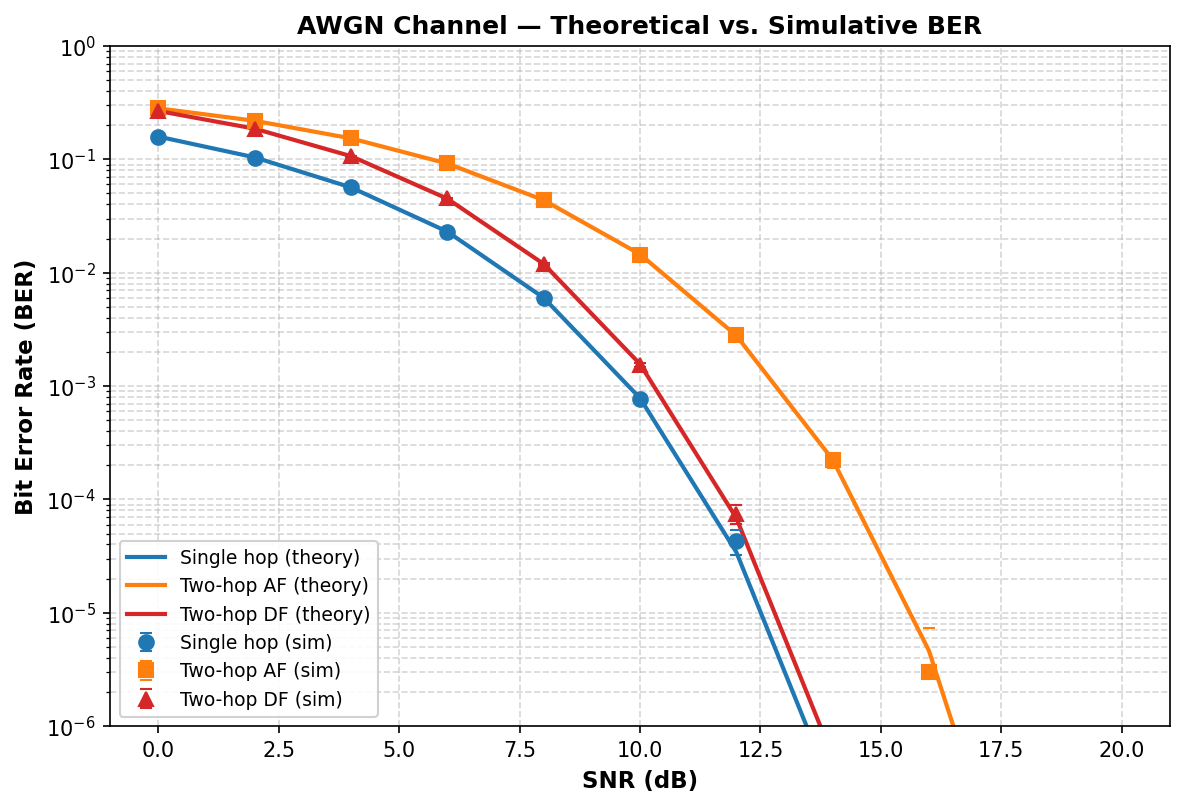
\includegraphics[width=\linewidth,height=0.8\textheight,keepaspectratio]{results/channel_theoretical_awgn.png}}
\caption{AWGN Channel : Theoretical vs.~Simulative BER. Single-hop, two-hop AF, and two-hop DF: closed-form theory (solid lines) versus Monte Carlo simulation (markers with 95\% CI). Theory and simulation match within the confidence interval at all SNR points.}
\end{figure}

\begin{figure}[H]
\centering
\centering
\pandocbounded{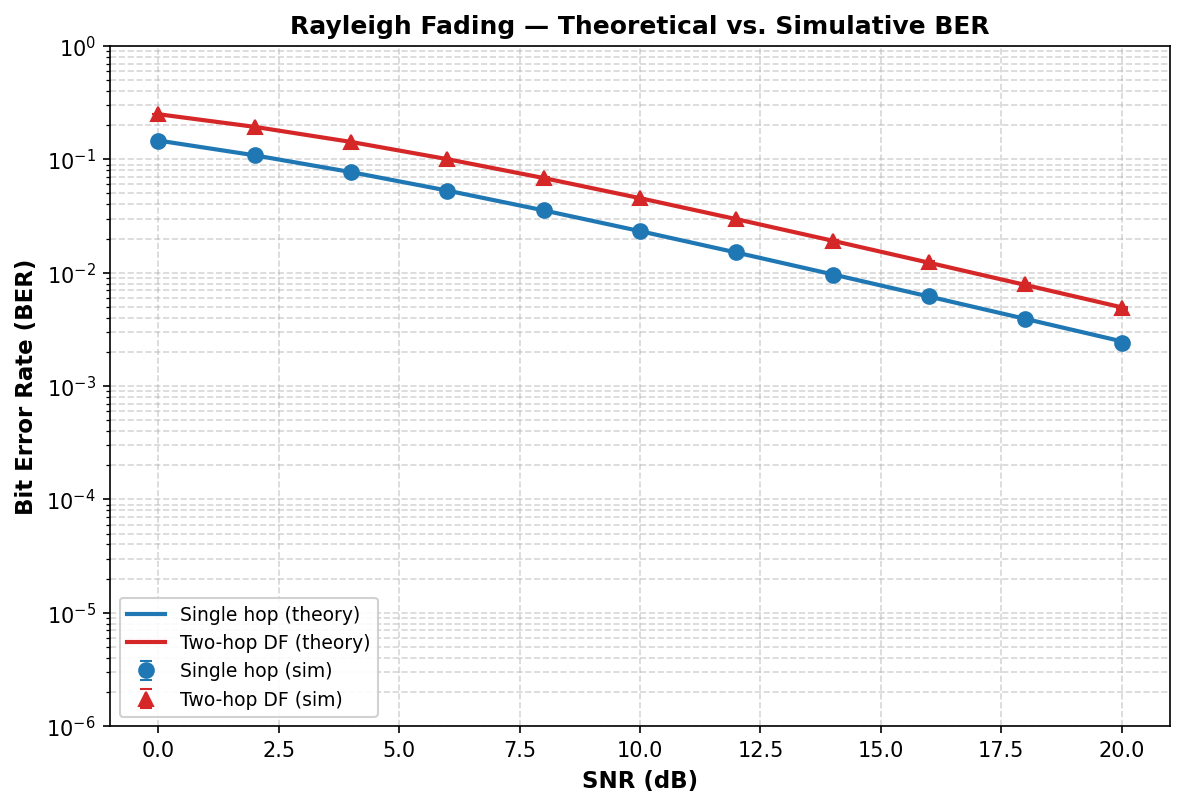
\includegraphics[width=\linewidth,height=0.8\textheight,keepaspectratio]{results/channel_theoretical_rayleigh.png}}
\caption{Rayleigh fading : theory vs.~simulation for single-hop and two-hop DF. The characteristic \(1/\text{SNR}\) slope (compared to the steeper exponential AWGN curve) is clearly visible.}
\end{figure}


\begin{figure}[H]
\centering
\centering
\pandocbounded{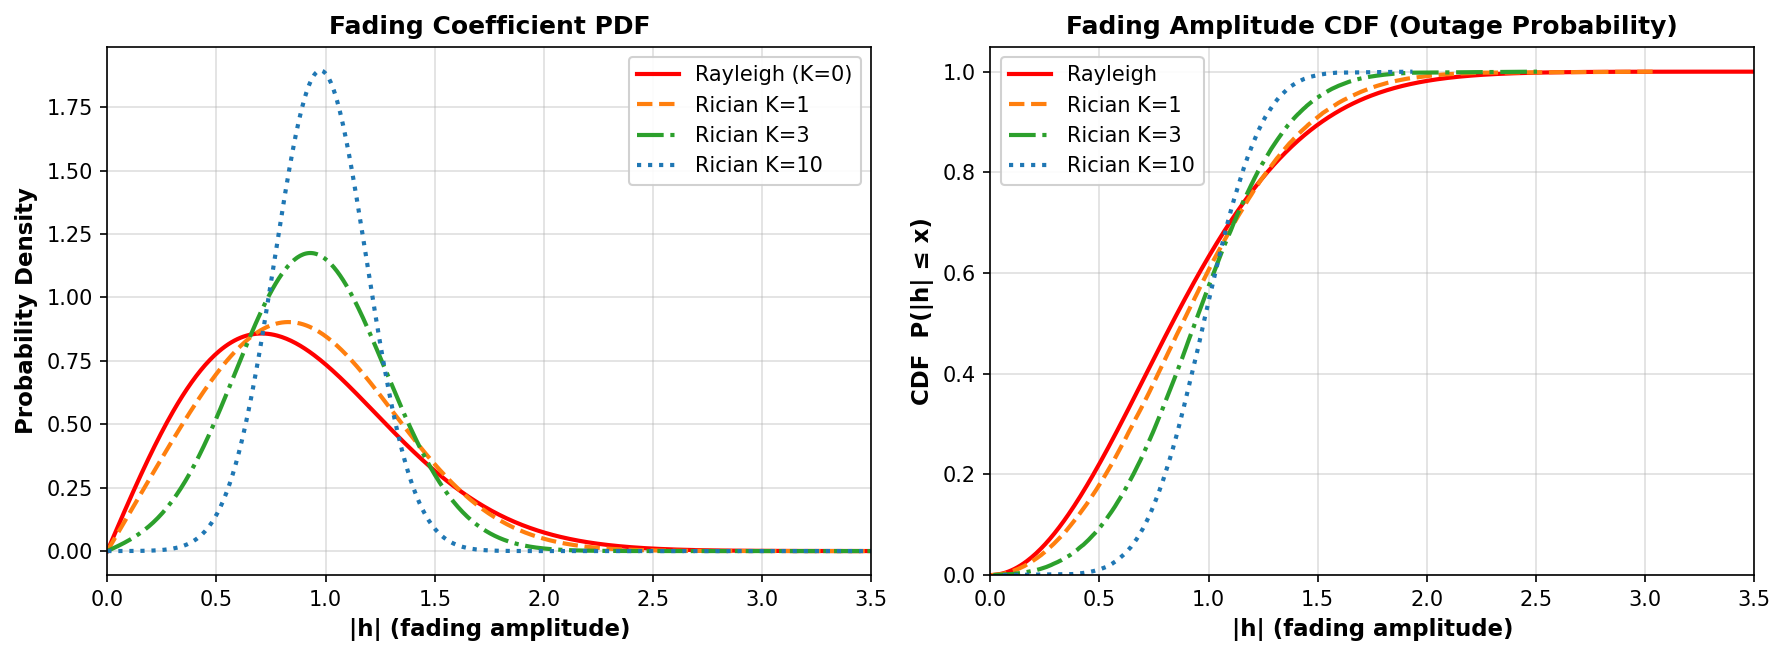
\includegraphics[width=\linewidth,height=0.8\textheight,keepaspectratio]{results/channel_fading_pdf.png}}
\caption{Left : PDF of \(|h|\) for Rayleigh and Rician (\(K=1, 3, 10\)). Right : CDF (outage probability). Rayleigh has the highest deep-fade probability at any threshold.}
\end{figure}






\section{Canonical Relay Comparison (SISO, Rayleigh, BPSK)}\label{sec:siso-bpsk-performance-baseline-relay-comparison}

\textbf{Goal:} Evaluate all nine classical and AI-based relay strategies on the canonical setup of this thesis.

\textbf{Trials:} - \textbf{Topology:} SISO (both hops) - \textbf{Modulation scheme:} BPSK - \textbf{Channel:} i.i.d.\ Rayleigh fast fading (canonical) - \textbf{Equalizers:} None - \textbf{NN architecture:} Supervised (MLP, Hybrid), Generative (VAE, CGAN), Sequence (Transformer, Mamba S6, Mamba-2 SSD) - \textbf{NN activation:} tanh

\textbf{Conclusion:} On the canonical Rayleigh channel, AI relays match but do not surpass symbol-wise DF: DF achieves the lowest or tied-lowest BER at essentially every SNR point, including the low-SNR regime, while the best neural relays (MLP, Hybrid, CGAN) track it within statistical uncertainty and clearly outperform AF. This confirms H1 (AI relays beat AF at low SNR) and H2 (DF dominance at $\geq 6$ dB with zero parameters) on the canonical channel.

\subsection{Results Tables}\label{sec:results-tables}


\begin{longtable}[]{@{}
  >{\raggedright\arraybackslash}p{(\linewidth - 18\tabcolsep) * \real{0.1000}}
  >{\raggedright\arraybackslash}p{(\linewidth - 18\tabcolsep) * \real{0.1000}}
  >{\raggedright\arraybackslash}p{(\linewidth - 18\tabcolsep) * \real{0.1000}}
  >{\raggedright\arraybackslash}p{(\linewidth - 18\tabcolsep) * \real{0.1000}}
  >{\raggedright\arraybackslash}p{(\linewidth - 18\tabcolsep) * \real{0.1000}}
  >{\raggedright\arraybackslash}p{(\linewidth - 18\tabcolsep) * \real{0.1000}}
  >{\raggedright\arraybackslash}p{(\linewidth - 18\tabcolsep) * \real{0.1000}}
  >{\raggedright\arraybackslash}p{(\linewidth - 18\tabcolsep) * \real{0.1000}}
  >{\raggedright\arraybackslash}p{(\linewidth - 18\tabcolsep) * \real{0.1000}}
  >{\raggedright\arraybackslash}p{(\linewidth - 18\tabcolsep) * \real{0.1000}}@{}}
\caption{BER comparison on the Rayleigh fading channel (SISO).}\label{tbl:table2}\tabularnewline
\toprule\noalign{}
\begin{minipage}[b]{\linewidth}\raggedright
SNR (dB)
\end{minipage} & \begin{minipage}[b]{\linewidth}\raggedright
AF
\end{minipage} & \begin{minipage}[b]{\linewidth}\raggedright
DF
\end{minipage} & \begin{minipage}[b]{\linewidth}\raggedright
MLP (169p)
\end{minipage} & \begin{minipage}[b]{\linewidth}\raggedright
Hybrid
\end{minipage} & \begin{minipage}[b]{\linewidth}\raggedright
VAE
\end{minipage} & \begin{minipage}[b]{\linewidth}\raggedright
CGAN
\end{minipage} & \begin{minipage}[b]{\linewidth}\raggedright
Trans-\\former
\end{minipage} & \begin{minipage}[b]{\linewidth}\raggedright
Mamba S6
\end{minipage} & \begin{minipage}[b]{\linewidth}\raggedright
Mamba2\\(ssd)
\end{minipage} \\
\midrule\noalign{}
\endfirsthead
\toprule\noalign{}
\begin{minipage}[b]{\linewidth}\raggedright
SNR (dB)
\end{minipage} & \begin{minipage}[b]{\linewidth}\raggedright
AF
\end{minipage} & \begin{minipage}[b]{\linewidth}\raggedright
DF
\end{minipage} & \begin{minipage}[b]{\linewidth}\raggedright
MLP (169p)
\end{minipage} & \begin{minipage}[b]{\linewidth}\raggedright
Hybrid
\end{minipage} & \begin{minipage}[b]{\linewidth}\raggedright
VAE
\end{minipage} & \begin{minipage}[b]{\linewidth}\raggedright
CGAN
\end{minipage} & \begin{minipage}[b]{\linewidth}\raggedright
Trans-\\former
\end{minipage} & \begin{minipage}[b]{\linewidth}\raggedright
Mamba(S6)
\end{minipage} & \begin{minipage}[b]{\linewidth}\raggedright
Mamba2(SSD)
\end{minipage} \\
\midrule\noalign{}
\endhead
\bottomrule\noalign{}
\endlastfoot
0 & 0.330 & \textbf{0.245} & 0.247 & 0.250 & 0.395 & 0.247 & 0.325 & 0.317 & 0.318 \\
4 & 0.205 & 0.139 & 0.141 & 0.141 & 0.347 & \textbf{0.138} & 0.183 & 0.178 & 0.180 \\
8 & 0.092 & \textbf{0.068} & 0.070 & 0.069 & 0.304 & 0.070 & 0.077 & 0.076 & 0.076 \\
12 & 0.037 & \textbf{0.031} & 0.032 & 0.032 & 0.278 & 0.031 & 0.032 & 0.032 & 0.032 \\
16 & 0.015 & 0.014 & 0.014 & 0.014 & 0.262 & 0.014 & 0.014 & \textbf{0.013} & 0.014 \\
20 & 0.0053 & \textbf{0.0047} & \textbf{0.0047} & \textbf{0.0047} & 0.250 & 0.0052 & 0.0048 & 0.0052 & \textbf{0.0047} \\
\end{longtable}


\subsection{Results Figures}\label{sec:results-figures-1}


\begin{figure}[H]
\centering
\centering
\pandocbounded{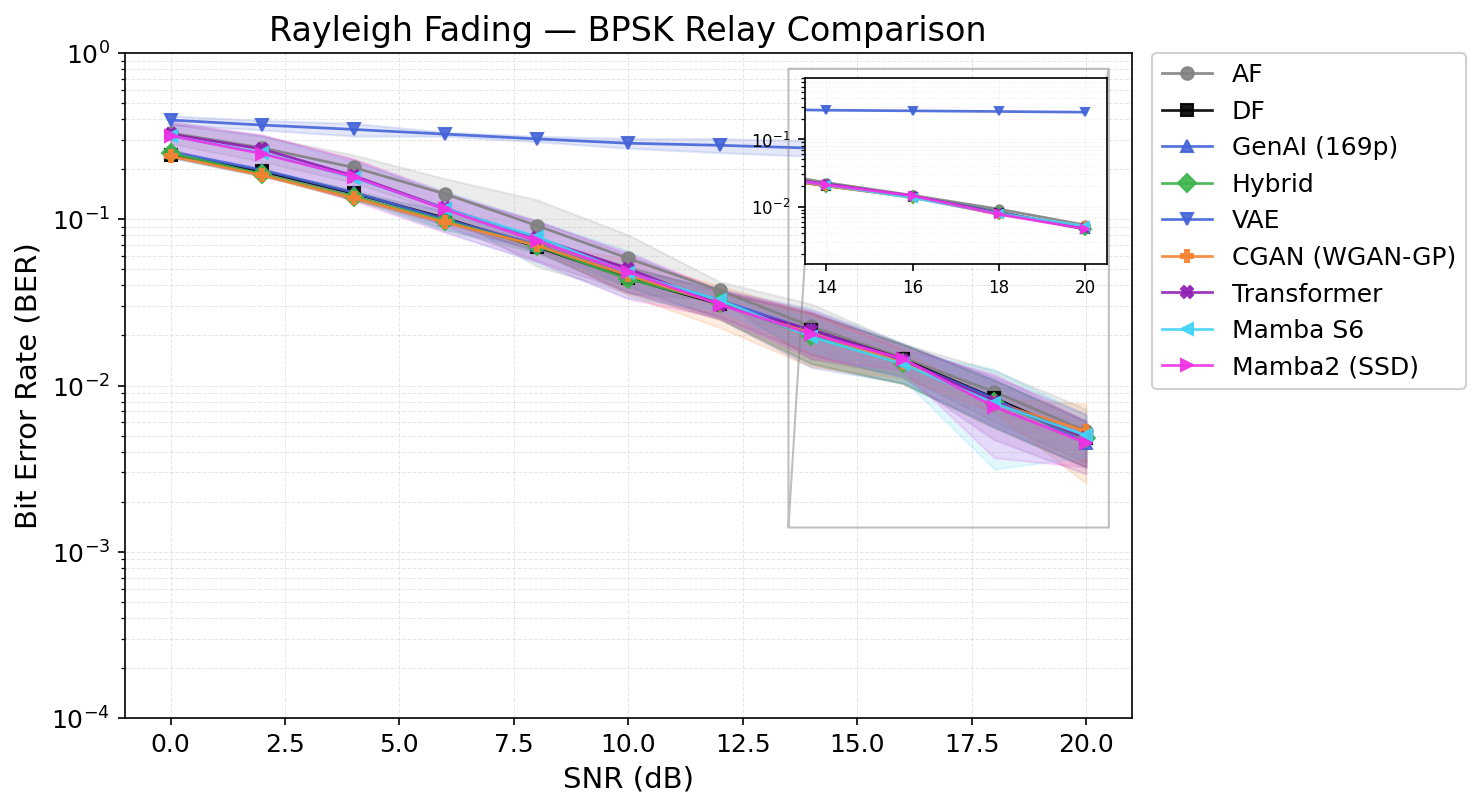
\includegraphics[width=\linewidth,height=0.8\textheight,keepaspectratio]{results/fading_comparison.png}}
\caption{Rayleigh fading : BER vs.~SNR for all nine relay strategies with 95\% CI.}\label{fig:fig10}
\end{figure}


\section{Parameter Normalization \& Complexity Trade-off}\label{sec:parameter-normalization-complexity-trade-off}

This study tests H3 (inverted-U complexity) and H4 (architecture convergence at equal scale) on the canonical setup, and provides the training-time benchmark for H5.

\textbf{Goal:} Isolate architectural inductive biases from parameter count effects and characterize the complexity-performance trade-off for relay denoising.

\textbf{Trials:} - \textbf{Topology:} SISO (both hops) - \textbf{Modulation scheme:} BPSK - \textbf{Channel:} i.i.d.\ Rayleigh fast fading (canonical) - \textbf{Equalizers:} None - \textbf{NN architecture:} All normalized to \textasciitilde3,000 parameters, plus original sizes (169 to 26K) - \textbf{NN activation:} tanh

\textbf{Conclusion:} The relay denoising task exhibits an inverted-U complexity relationship: a minimal 169-parameter MLP matches models 140x larger, while excessive parameters (11K+) lead to overfitting. At a normalized scale of 3,000 parameters, the performance gap between feedforward and sequence architectures narrows to \textasciitilde1\% BER, indicating that parameter count rather than architectural choice is the primary performance driver. Generative VAE is a consistent underperformer due to probabilistic overhead.

\subsection{Results Tables}\label{sec:results-tables-2}


\begin{longtable}[]{@{}
  >{\raggedright\arraybackslash}p{(\linewidth - 16\tabcolsep) * \real{0.1111}}
  >{\raggedright\arraybackslash}p{(\linewidth - 16\tabcolsep) * \real{0.1111}}
  >{\raggedright\arraybackslash}p{(\linewidth - 16\tabcolsep) * \real{0.1111}}
  >{\raggedright\arraybackslash}p{(\linewidth - 16\tabcolsep) * \real{0.1111}}
  >{\raggedright\arraybackslash}p{(\linewidth - 16\tabcolsep) * \real{0.1111}}
  >{\raggedright\arraybackslash}p{(\linewidth - 16\tabcolsep) * \real{0.1111}}
  >{\raggedright\arraybackslash}p{(\linewidth - 16\tabcolsep) * \real{0.1111}}
  >{\raggedright\arraybackslash}p{(\linewidth - 16\tabcolsep) * \real{0.1111}}
  >{\raggedright\arraybackslash}p{(\linewidth - 16\tabcolsep) * \real{0.1111}}@{}}
\caption{Normalized 3K BER results : Rayleigh fading channel.}\label{tbl:table8}\tabularnewline
\toprule\noalign{}
\begin{minipage}[b]{\linewidth}\raggedright
SNR (dB)
\end{minipage} & \begin{minipage}[b]{\linewidth}\raggedright
MLP-3K
\end{minipage} & \begin{minipage}[b]{\linewidth}\raggedright
Hybrid-3K
\end{minipage} & \begin{minipage}[b]{\linewidth}\raggedright
VAE-3K
\end{minipage} & \begin{minipage}[b]{\linewidth}\raggedright
Trans-\\former\\(3K)
\end{minipage} & \begin{minipage}[b]{\linewidth}\raggedright
Mamba\\(3K)
\end{minipage} & \begin{minipage}[b]{\linewidth}\raggedright
Mamba2\\(3K)
\end{minipage} & \begin{minipage}[b]{\linewidth}\raggedright
AF
\end{minipage} & \begin{minipage}[b]{\linewidth}\raggedright
DF
\end{minipage} \\
\midrule\noalign{}
\endfirsthead
\toprule\noalign{}
\begin{minipage}[b]{\linewidth}\raggedright
SNR (dB)
\end{minipage} & \begin{minipage}[b]{\linewidth}\raggedright
MLP-3K
\end{minipage} & \begin{minipage}[b]{\linewidth}\raggedright
Hybrid-3K
\end{minipage} & \begin{minipage}[b]{\linewidth}\raggedright
VAE-3K
\end{minipage} & \begin{minipage}[b]{\linewidth}\raggedright
Trans-\\former\\(3K)
\end{minipage} & \begin{minipage}[b]{\linewidth}\raggedright
Mamba\\(3K)
\end{minipage} & \begin{minipage}[b]{\linewidth}\raggedright
Mamba2\\(3K)
\end{minipage} & \begin{minipage}[b]{\linewidth}\raggedright
AF
\end{minipage} & \begin{minipage}[b]{\linewidth}\raggedright
DF
\end{minipage} \\
\midrule\noalign{}
\endhead
\bottomrule\noalign{}
\endlastfoot
0 & \textbf{0.252} & 0.258 & 0.411 & 0.329 & 0.320 & 0.320 & 0.330 & 0.245 \\
4 & 0.146 & \textbf{0.145} & 0.375 & 0.181 & 0.180 & 0.179 & 0.205 & 0.139 \\
10 & 0.049 & \textbf{0.047} & 0.315 & 0.050 & 0.049 & 0.049 & 0.058 & 0.044 \\
16 & 0.015 & 0.014 & 0.289 & 0.014 & \textbf{0.014} & 0.014 & 0.015 & 0.014 \\
20 & 0.0050 & \textbf{0.0047} & 0.279 & \textbf{0.0047} & \textbf{0.0047} & \textbf{0.0047} & 0.0053 & 0.0047 \\
\end{longtable}





\begin{longtable}[]{@{}
  >{\raggedright\arraybackslash}p{(\linewidth - 8\tabcolsep) * \real{0.28}}
  >{\raggedright\arraybackslash}p{(\linewidth - 8\tabcolsep) * \real{0.15}}
  >{\raggedright\arraybackslash}p{(\linewidth - 8\tabcolsep) * \real{0.12}}
  >{\raggedright\arraybackslash}p{(\linewidth - 8\tabcolsep) * \real{0.27}}
  >{\raggedright\arraybackslash}p{(\linewidth - 8\tabcolsep) * \real{0.18}}@{}}
\caption{Model complexity and timing comparison on the canonical setup (experiment-specific training settings; Monte Carlo evaluation over 11 SNR points x 10 trials x 10,000 bits). All inference uses batched window extraction and a single forward pass per signal block.}\label{tbl:table13}\tabularnewline
\toprule\noalign{}
Model & Parameters & Device & Training Time & Eval Time \\
\midrule\noalign{}
\endfirsthead
\toprule\noalign{}
Model & Parameters & Device & Training Time & Eval Time \\
\midrule\noalign{}
\endhead
\bottomrule\noalign{}
\endlastfoot
AF & 0 & : & 0 s & 0.80 s \\
DF & 0 & : & 0 s & 0.77 s \\
MLP (169p) & 169 & CPU & 4.9 s & 1.57 s \\
Hybrid & 169 & CPU & 4.6 s & 0.41 s \\
VAE & 1,777 & CPU & 21.6 s & 1.81 s \\
CGAN (WGAN-GP) & 2,946 & CUDA & 7,293 s (\textasciitilde2 h) & 1.14 s \\
Transformer & 17,697 & CUDA & 474 s (\textasciitilde8 min) & 3.71 s \\
\textbf{Mamba S6} & \textbf{24,001} & \textbf{CUDA} & \textbf{2,141 s (\textasciitilde36 min)} & \textbf{1.88 s} \\
\textbf{Mamba2 (SSD)} & \textbf{26,179} & \textbf{CUDA} & \textbf{1,438 s (\textasciitilde24 min)} & \textbf{4.11 s} \\
\end{longtable}

\subsection{Results Figures}\label{sec:results-figures-3}



\begin{figure}[H]
\centering
\centering
\pandocbounded{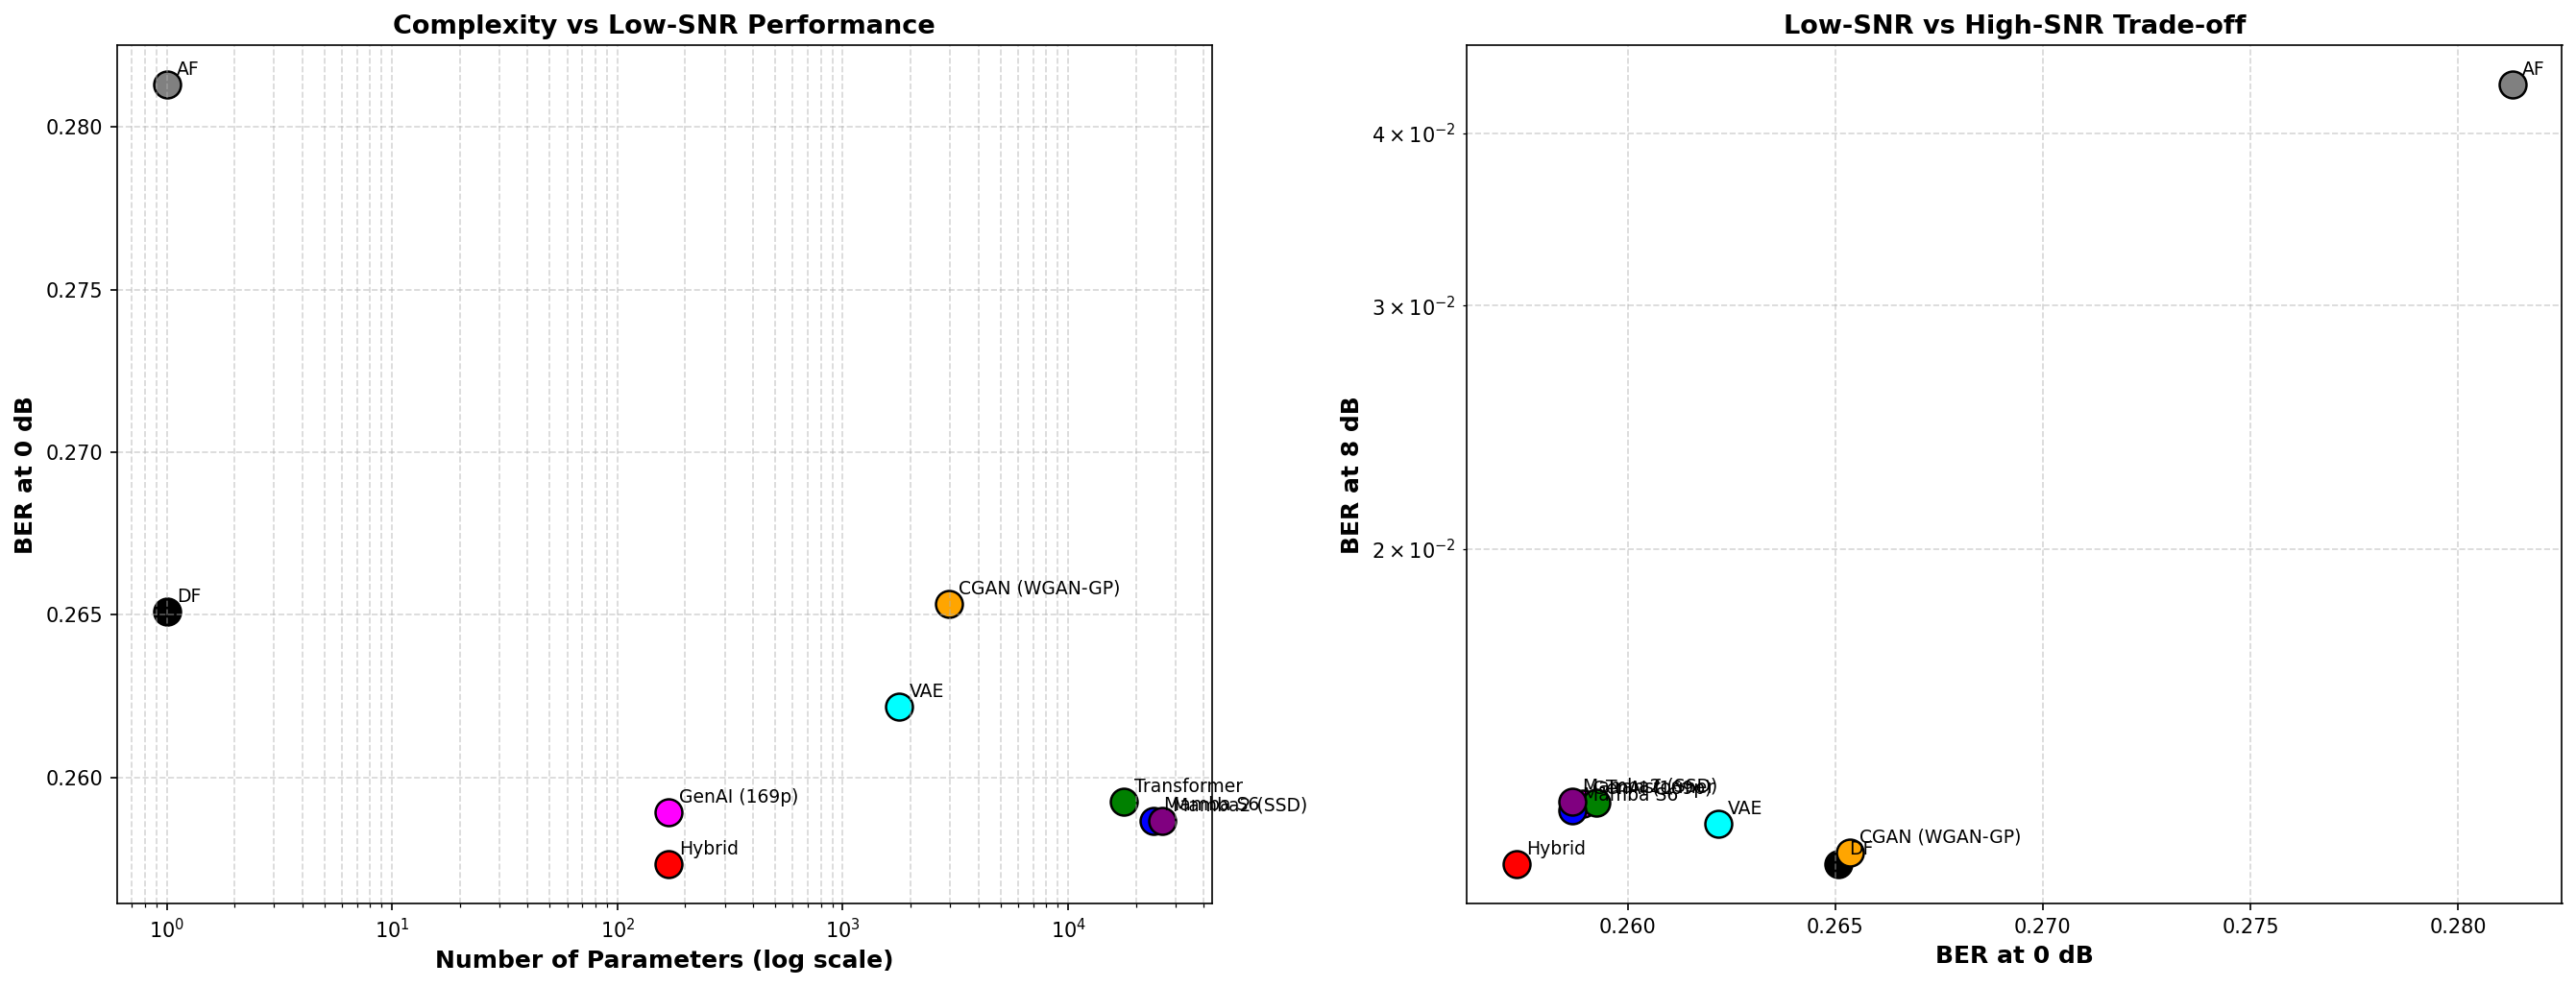
\includegraphics[width=\linewidth,height=0.8\textheight,keepaspectratio]{results/complexity_comparison_all_relays.png}}
\caption{Complexity--performance trade-off. Training time vs.~parameter count vs.~BER improvement over DF at low SNR. The Minimal MLP (169 params) achieves the best efficiency.}\label{fig:fig19}
\end{figure}

\chapter{Extension: Higher-Order Modulations}\label{sec:extensions}

The core of this thesis (Chapter~\ref{sec:experiments}) answers hypotheses H1--H5 on the canonical setup. This chapter contains one scoped extension: whether the canonical BPSK conclusions generalize to complex constellations. Two studies are reported. The first evaluates QPSK and 16-QAM under the I/Q-splitting formulation, exposing a structural BER floor for multi-level constellations; the second removes that floor by reformulating the relay as a joint $N$-class classifier over the full 2D constellation ($N=16$ for 16-QAM). These analyses adopt the channel configurations under which they were conducted (AWGN and Rayleigh for the first study, AWGN for the second); MIMO, 16-PSK, CSI injection, and end-to-end learning remain future work. The separate question of how classical and learned relays behave when the \emph{channel itself} is unknown or mismatched --- a more substantial investigation --- forms the dedicated contribution of Chapter~\ref{sec:unknown-channels}.

\section{Higher-Order Modulation Scalability (Constellation-Aware Training)}\label{sec:higher-order-modulation-scalability-constellation-aware-training}

\textbf{Goal:} Evaluate the generalizability of BPSK-trained relays to complex constellations and resolve the multi-level amplitude bottleneck.

\textbf{Trials:} - \textbf{Topology:} SISO - \textbf{Modulation scheme:} QPSK, 16-QAM - \textbf{Channel:} AWGN, Rayleigh - \textbf{Equalizers:} None - \textbf{NN architecture:} Supervised (MLP, Hybrid), Generative (VAE, CGAN), Sequence (Transformer, Mamba S6, Mamba-2 SSD) - \textbf{NN activation:} tanh, linear, clipped tanh (hardtanh), scaled tanh, scaled sigmoid - \textbf{Special case:} Constellation Aware training

\textbf{Conclusion:} QPSK performance mirrors BPSK perfectly due to I/Q independence. On 16-QAM, standard tanh compression causes a severe, irreducible BER floor (\textasciitilde0.22 at 16 dB). Replacing tanh with constellation-aware bounded activations (hardtanh, scaled tanh) bounded to the precise signal amplitude (\(3/\sqrt{10}\)) and retraining eliminates this floor. Sequence models benefit most, reducing their BER floor by 5x, though a gap to classical DF persists due to per-axis error accumulation --- the limitation removed by the 2D classification study below.

\subsection{Results Tables}\label{sec:results-tables-3}

\begin{longtable}[]{@{}
  >{\raggedright\arraybackslash}p{(\linewidth - 14\tabcolsep) * \real{0.1250}}
  >{\raggedright\arraybackslash}p{(\linewidth - 14\tabcolsep) * \real{0.1250}}
  >{\raggedright\arraybackslash}p{(\linewidth - 14\tabcolsep) * \real{0.1250}}
  >{\raggedright\arraybackslash}p{(\linewidth - 14\tabcolsep) * \real{0.1250}}
  >{\raggedright\arraybackslash}p{(\linewidth - 14\tabcolsep) * \real{0.1250}}
  >{\raggedright\arraybackslash}p{(\linewidth - 14\tabcolsep) * \real{0.1250}}
  >{\raggedright\arraybackslash}p{(\linewidth - 14\tabcolsep) * \real{0.1250}}
  >{\raggedright\arraybackslash}p{(\linewidth - 14\tabcolsep) * \real{0.1250}}@{}}
\caption{BER comparison across modulations at selected SNR points (AWGN channel). All nine relay strategies.}\label{tbl:table14}\tabularnewline
\toprule\noalign{}
\begin{minipage}[b]{\linewidth}\raggedright
Relay
\end{minipage} & \begin{minipage}[b]{\linewidth}\raggedright
BPSK 0 dB
\end{minipage} & \begin{minipage}[b]{\linewidth}\raggedright
BPSK 10 dB
\end{minipage} & \begin{minipage}[b]{\linewidth}\raggedright
QPSK 0 dB
\end{minipage} & \begin{minipage}[b]{\linewidth}\raggedright
QPSK 10 dB
\end{minipage} & \begin{minipage}[b]{\linewidth}\raggedright
16-QAM 0 dB
\end{minipage} & \begin{minipage}[b]{\linewidth}\raggedright
16-QAM 10 dB
\end{minipage} & \begin{minipage}[b]{\linewidth}\raggedright
16-QAM 16 dB
\end{minipage} \\
\midrule\noalign{}
\endfirsthead
\toprule\noalign{}
\begin{minipage}[b]{\linewidth}\raggedright
Relay
\end{minipage} & \begin{minipage}[b]{\linewidth}\raggedright
BPSK 0 dB
\end{minipage} & \begin{minipage}[b]{\linewidth}\raggedright
BPSK 10 dB
\end{minipage} & \begin{minipage}[b]{\linewidth}\raggedright
QPSK 0 dB
\end{minipage} & \begin{minipage}[b]{\linewidth}\raggedright
QPSK 10 dB
\end{minipage} & \begin{minipage}[b]{\linewidth}\raggedright
16-QAM 0 dB
\end{minipage} & \begin{minipage}[b]{\linewidth}\raggedright
16-QAM 10 dB
\end{minipage} & \begin{minipage}[b]{\linewidth}\raggedright
16-QAM 16 dB
\end{minipage} \\
\midrule\noalign{}
\endhead
\bottomrule\noalign{}
\endlastfoot
AF & 0.2813 & 0.0141 & 0.2794 & 0.0142 & 0.3778 & 0.1244 & 0.0180 \\
DF & 0.2651 & 0.0015 & 0.2644 & 0.0016 & 0.3811 & 0.1076 & 0.0038 \\
MLP (169p) & 0.2589 & 0.0021 & 0.2563 & 0.0025 & 0.3907 & 0.2180 & 0.2180 \\
Hybrid & 0.2573 & 0.0015 & 0.2644 & 0.0016 & 0.4000 & 0.2711 & 0.2512 \\
VAE & 0.2611 & 0.0021 & 0.2597 & 0.0036 & 0.3945 & 0.2391 & 0.2231 \\
CGAN (WGAN-GP) & 0.2633 & 0.0017 & 0.2621 & 0.0018 & 0.3976 & 0.2588 & 0.2486 \\
trans-\\former & 0.2593 & 0.0024 & 0.2576 & 0.0036 & 0.3897 & 0.2042 & 0.1827 \\
Mamba S6 & 0.2585 & 0.0021 & 0.2560 & 0.0028 & 0.3894 & 0.2016 & 0.1935 \\
Mamba2 (SSD) & 0.2593 & 0.0023 & 0.2566 & 0.0034 & 0.3903 & 0.2032 & 0.1890 \\
\end{longtable}

Table 15 shows the BER at 16 dB for all relays across the three activation variants and both channel types.

\begin{longtable}[]{@{}
  >{\raggedright\arraybackslash}p{(\linewidth - 12\tabcolsep) * \real{0.1429}}
  >{\raggedright\arraybackslash}p{(\linewidth - 12\tabcolsep) * \real{0.1429}}
  >{\raggedright\arraybackslash}p{(\linewidth - 12\tabcolsep) * \real{0.1429}}
  >{\raggedright\arraybackslash}p{(\linewidth - 12\tabcolsep) * \real{0.1429}}
  >{\raggedright\arraybackslash}p{(\linewidth - 12\tabcolsep) * \real{0.1429}}
  >{\raggedright\arraybackslash}p{(\linewidth - 12\tabcolsep) * \real{0.1429}}
  >{\raggedright\arraybackslash}p{(\linewidth - 12\tabcolsep) * \real{0.1429}}@{}}
\caption{BER at 16 dB for all relay variants across activation functions and modulations (AWGN and Rayleigh).}\label{tbl:table15}\tabularnewline
\toprule\noalign{}
\begin{minipage}[b]{\linewidth}\raggedright
Relay
\end{minipage} & \begin{minipage}[b]{\linewidth}\raggedright
tanh (BPSK)
\end{minipage} & \begin{minipage}[b]{\linewidth}\raggedright
linear (QAM16)
\end{minipage} & \begin{minipage}[b]{\linewidth}\raggedright
hardtanh (QAM16)
\end{minipage} & \begin{minipage}[b]{\linewidth}\raggedright
tanh (BPSK)
\end{minipage} & \begin{minipage}[b]{\linewidth}\raggedright
linear (QAM16)
\end{minipage} & \begin{minipage}[b]{\linewidth}\raggedright
hardtanh (QAM16)
\end{minipage} \\
\midrule\noalign{}
\endfirsthead
\toprule\noalign{}
\begin{minipage}[b]{\linewidth}\raggedright
Relay
\end{minipage} & \begin{minipage}[b]{\linewidth}\raggedright
tanh (BPSK)
\end{minipage} & \begin{minipage}[b]{\linewidth}\raggedright
linear (QAM16)
\end{minipage} & \begin{minipage}[b]{\linewidth}\raggedright
hardtanh (QAM16)
\end{minipage} & \begin{minipage}[b]{\linewidth}\raggedright
tanh (BPSK)
\end{minipage} & \begin{minipage}[b]{\linewidth}\raggedright
linear (QAM16)
\end{minipage} & \begin{minipage}[b]{\linewidth}\raggedright
hardtanh (QAM16)
\end{minipage} \\
\midrule\noalign{}
\endhead
\bottomrule\noalign{}
\endlastfoot
& \textbf{AWGN} & & & \textbf{Rayleigh} & & \\
MLP & 0.2202 & 0.0721 & \textbf{0.0630} & 0.2375 & 0.1279 & \textbf{0.1247} \\
Hybrid & 0.2512 & 0.2512 & 0.2512 & 0.2723 & 0.2723 & 0.2723 \\
VAE & 0.2231 & 0.1111 & \textbf{0.1059} & 0.2462 & 0.1575 & \textbf{0.1573} \\
CGAN & 0.2482 & 0.0973 & \textbf{0.0863} & 0.2666 & 0.1432 & \textbf{0.1383} \\
trans-\\former & 0.2111 & \textbf{0.0453} & 0.0505 & 0.2305 & \textbf{0.1159} & 0.1194 \\
Mamba S6 & 0.2131 & 0.0422 & \textbf{0.0396} & 0.2333 & 0.1129 & \textbf{0.1108} \\
Mamba2\\(ssd) & 0.2065 & 0.0471 & \textbf{0.0441} & 0.2273 & 0.1157 & \textbf{0.1145} \\
AF & 0.0180 & : & : & 0.1009 & : & : \\
DF & 0.0038 & : & : & 0.0828 & : & : \\
\end{longtable}

Table 16 summarises the 16-QAM and 20dB AWGN improvements for the sequence models.

\begin{longtable}[]{@{}
  >{\raggedright\arraybackslash}p{(\linewidth - 8\tabcolsep) * \real{0.2000}}
  >{\raggedright\arraybackslash}p{(\linewidth - 8\tabcolsep) * \real{0.2000}}
  >{\raggedright\arraybackslash}p{(\linewidth - 8\tabcolsep) * \real{0.2000}}
  >{\raggedright\arraybackslash}p{(\linewidth - 8\tabcolsep) * \real{0.2000}}
  >{\raggedright\arraybackslash}p{(\linewidth - 8\tabcolsep) * \real{0.2000}}@{}}
\caption{16-QAM BER improvements at 20 dB for sequence models with and without CSI injection and layer normalisation (AWGN).}\label{tbl:table16}\tabularnewline
\toprule\noalign{}
\begin{minipage}[b]{\linewidth}\raggedright
SNR (dB)
\end{minipage} & \begin{minipage}[b]{\linewidth}\raggedright
AF Baseline
\end{minipage} & \begin{minipage}[b]{\linewidth}\raggedright
DF Baseline
\end{minipage} & \begin{minipage}[b]{\linewidth}\raggedright
Mamba S6 (Baseline)
\end{minipage} & \begin{minipage}[b]{\linewidth}\raggedright
Mamba S6 (+CSI + LN)
\end{minipage} \\
\midrule\noalign{}
\endfirsthead
\toprule\noalign{}
\begin{minipage}[b]{\linewidth}\raggedright
SNR (dB)
\end{minipage} & \begin{minipage}[b]{\linewidth}\raggedright
AF Baseline
\end{minipage} & \begin{minipage}[b]{\linewidth}\raggedright
DF Baseline
\end{minipage} & \begin{minipage}[b]{\linewidth}\raggedright
Mamba S6 (Baseline)
\end{minipage} & \begin{minipage}[b]{\linewidth}\raggedright
Mamba S6 (+CSI + LN)
\end{minipage} \\
\midrule\noalign{}
\endhead
\bottomrule\noalign{}
\endlastfoot
\textbf{0.0} & 0.3332 & 0.4300 & 0.2288 & 0.2396 \\
\textbf{8.0} & 0.1436 & 0.2798 & 0.2241 & 0.0635 \\
\textbf{14.0} & 0.0592 & 0.1557 & 0.2227 & 0.0163 \\
\textbf{20.0} & 0.0246 & 0.0901 & 0.2302 & \textbf{0.0055} \\
\end{longtable}

\subsection{Results Figures}\label{sec:results-figures-4}

\begin{figure}[H]
\centering
\centering
\pandocbounded{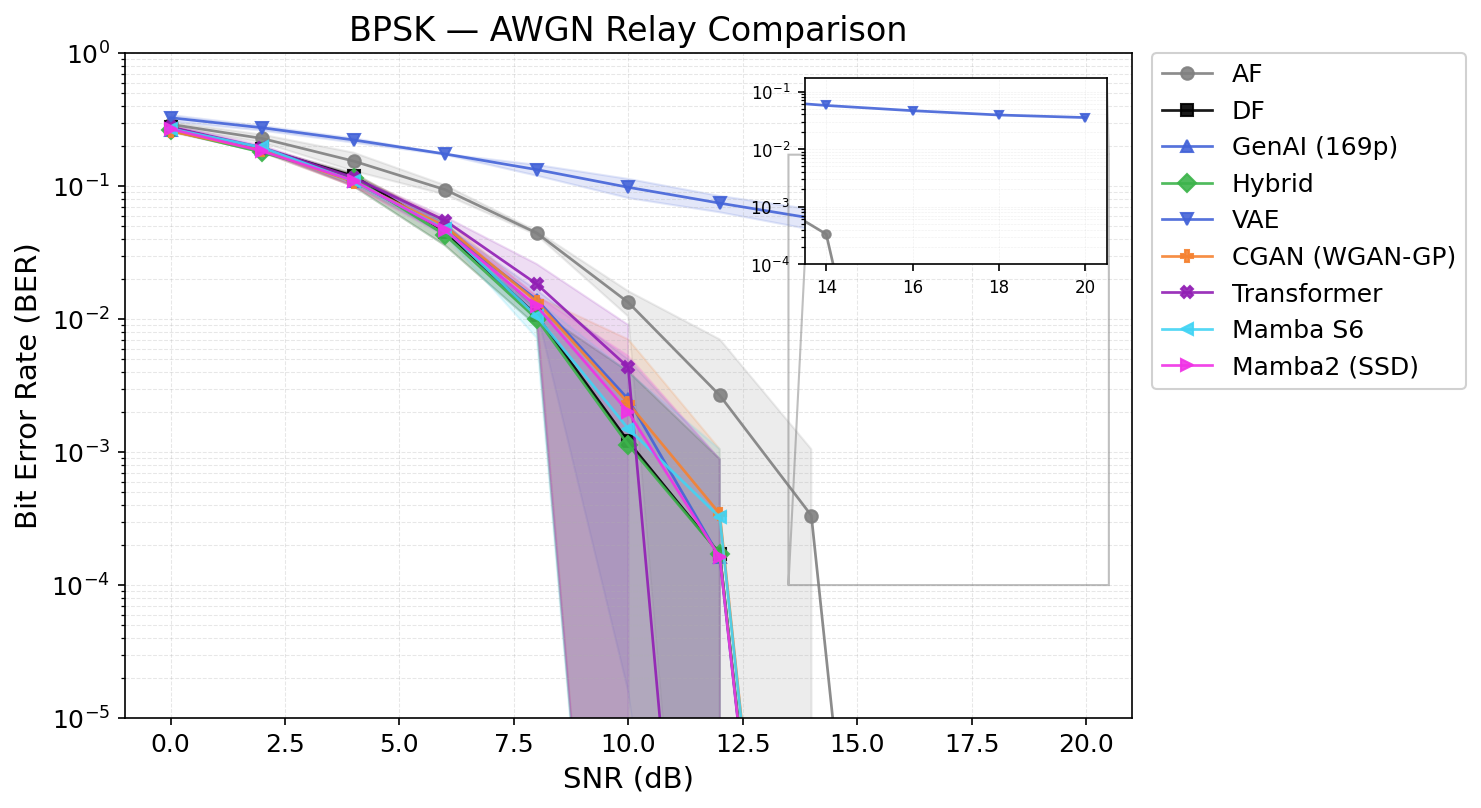
\includegraphics[width=\linewidth,height=0.8\textheight,keepaspectratio]{results/modulation/bpsk_awgn_ci.png}}
\caption{BPSK on AWGN : all relay strategies with 95\% CI (baseline for modulation comparison).}\label{fig:fig21}
\end{figure}

\begin{figure}[H]
\centering
\centering
\pandocbounded{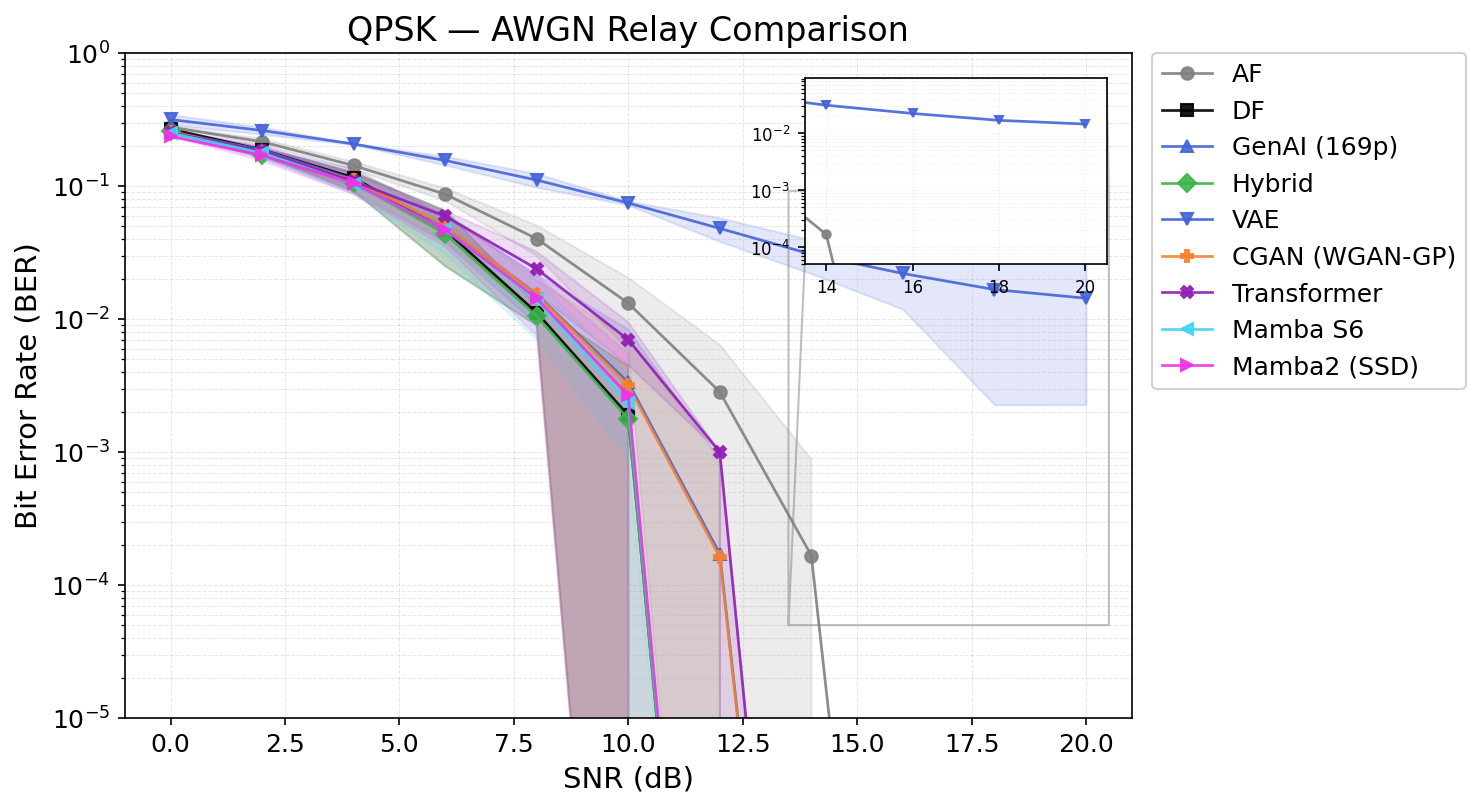
\includegraphics[width=\linewidth,height=0.8\textheight,keepaspectratio]{results/modulation/qpsk_awgn_ci.png}}
\caption{QPSK on AWGN : BER curves closely match the BPSK baseline (\ref{fig:fig21}), confirming I/Q splitting validity.}\label{fig:fig23}
\end{figure}

\begin{figure}[H]
\centering
\centering
\pandocbounded{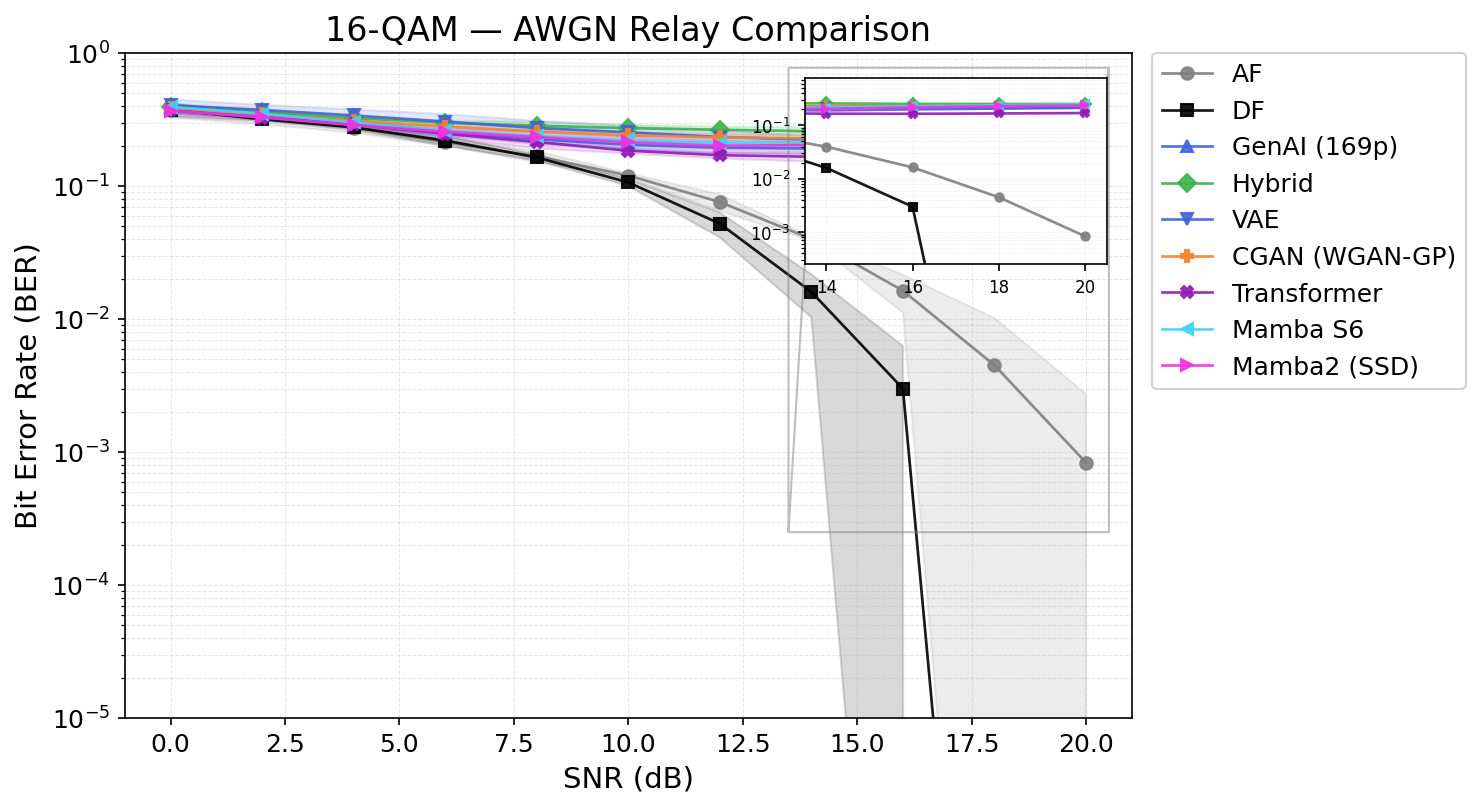
\includegraphics[width=\linewidth,height=0.8\textheight,keepaspectratio]{results/modulation/qam16__awgn_ci.png}}
\caption{16-QAM on AWGN : AI relays hit a BER floor near 0.22 at medium-high SNR due to \(\tanh\) compression of multi-level signals; AF outperforms DF at low SNR (Y}\label{fig:fig25}
\end{figure}

\begin{figure}[H]
\centering
\centering
\pandocbounded{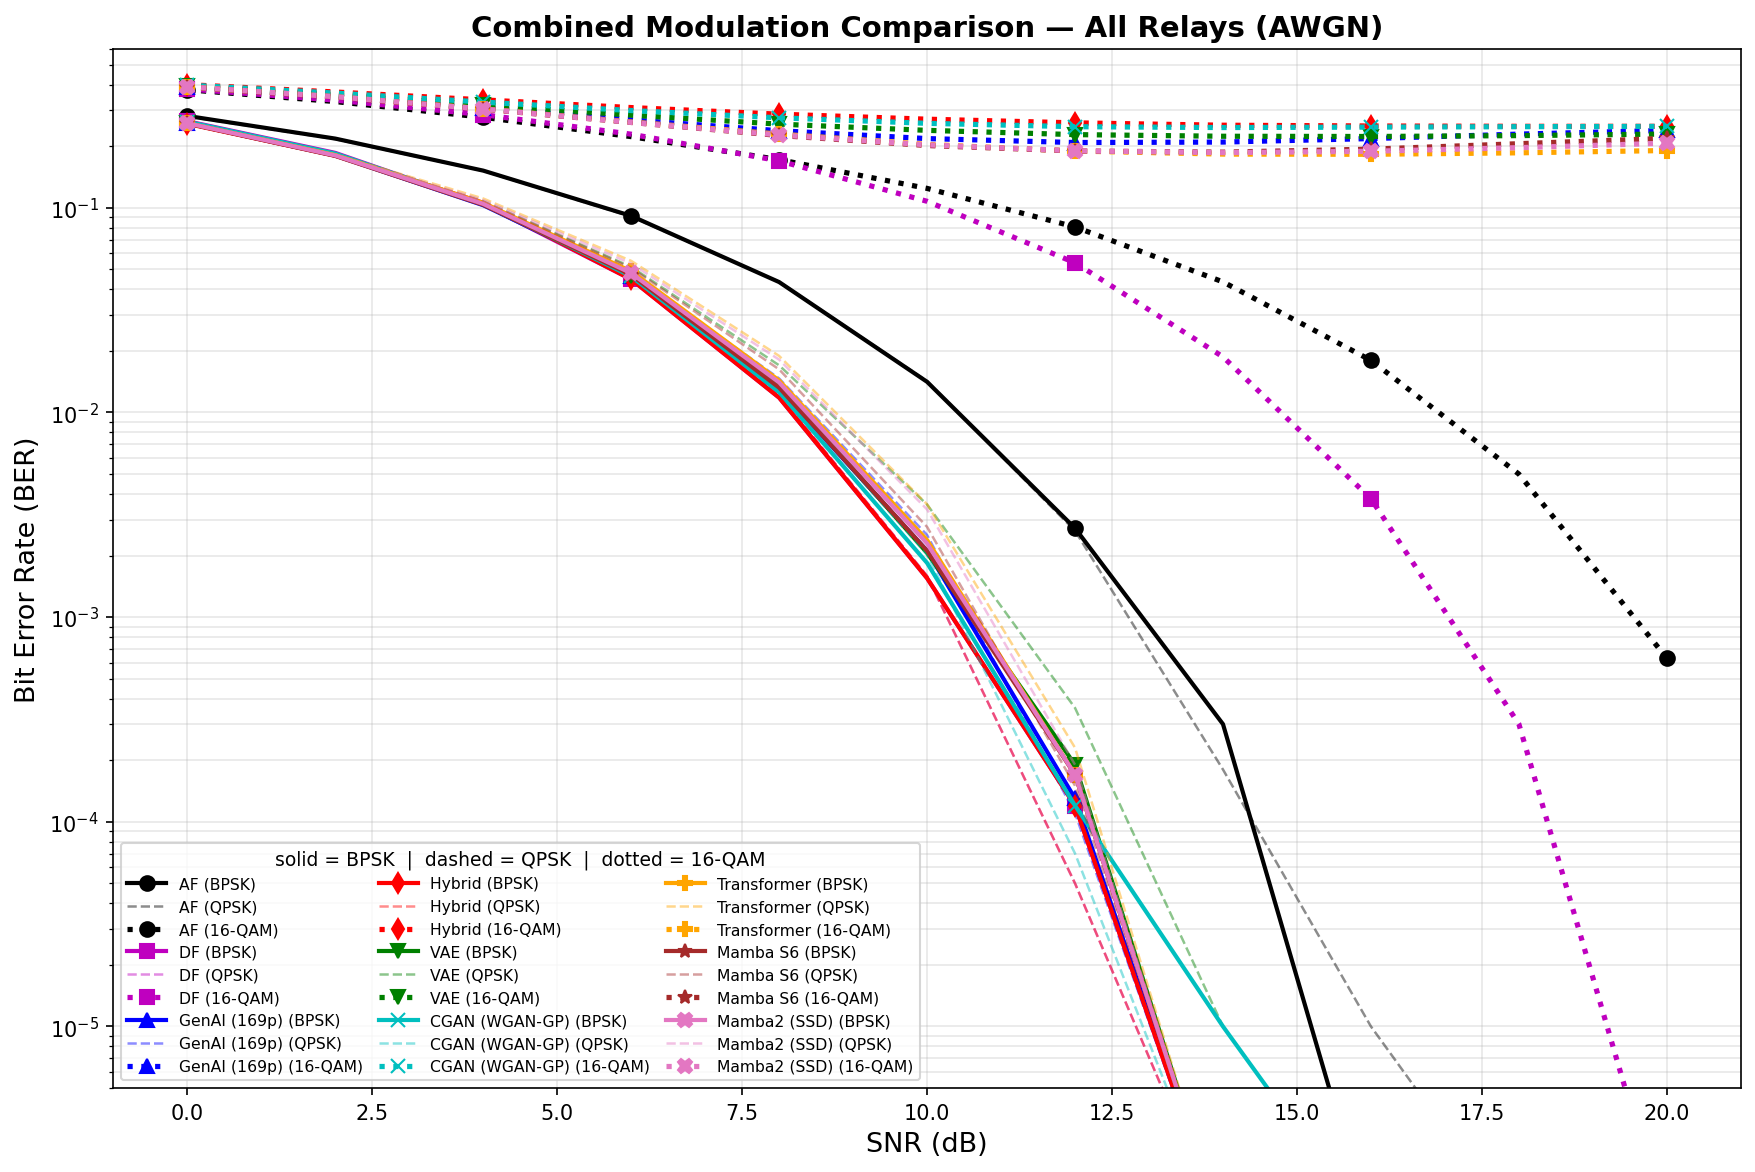
\includegraphics[width=\linewidth,height=0.8\textheight,keepaspectratio]{results/modulation/combined_modulation_awgn.png}}
\caption{Combined modulation comparison (AWGN) : all nine relays across BPSK (solid), QPSK (dashed, overlapping BPSK), and 16-QAM (dotted). The BPSK/QPSK overlap confirms I/Q splitting equivalence. The 16-QAM dotted curves reveal the AI relay BER floor: all AI relays plateau near 0.18--0.25 while DF and AF continue decreasing.}\label{fig:fig27}
\end{figure}

\begin{figure}[H]
\centering
\centering
\pandocbounded{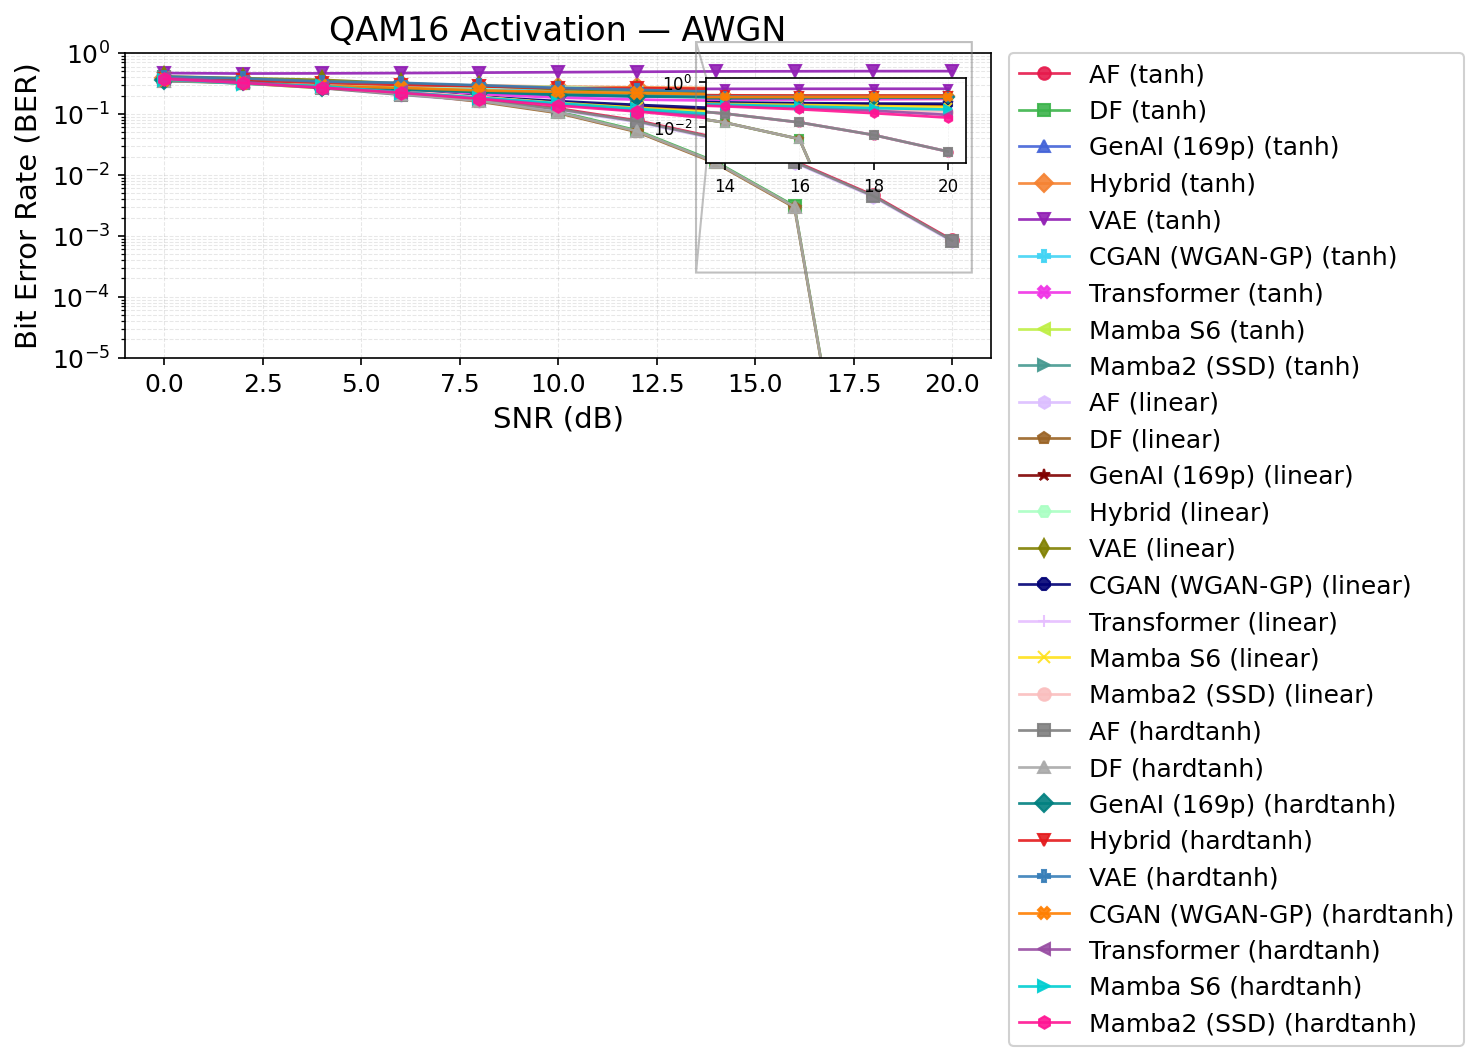
\includegraphics[width=\linewidth,height=0.8\textheight,keepaspectratio]{results/qam16_activation/qam16_activation_awgn.png}}
\caption{16-QAM activation experiment (AWGN) : dashed lines = tanh/BPSK baseline, solid = linear/QAM16, dotted = hardtanh/QAM16. Replacing tanh and retraining on QAM16 eliminates the BER floor for all AI relays except Hybrid. Sequence models (Transformer, Mamba S6, Mamba-2) benefit most, narrowing the gap to DF from \textasciitilde56x to \textasciitilde10x.}\label{fig:fig28}
\end{figure}

\begin{figure}[H]
\centering
\centering
\pandocbounded{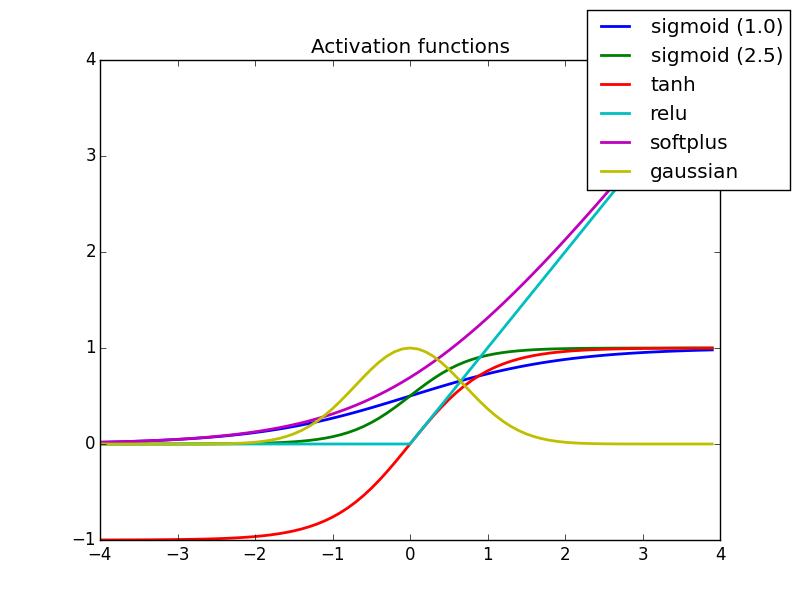
\includegraphics[width=\linewidth,height=0.8\textheight,keepaspectratio]{results/activation_comparison/various_activation_functions.png}}
\caption{Comparison of activation function shapes (left) and their derivatives (right) for \(A_{\max} = 0.9487\) (16-QAM). Hardtanh has a sharp transition at the clip bounds; sigmoid and scaled tanh provide smooth saturation with non-zero gradients throughout.}\label{fig:fig36}
\end{figure}


\section{16-Class 2D Classification for QAM16}\label{sec:class-2d-classification-for-qam16}

\textbf{Goal:} Eliminate the structural BER floor imposed by per-axis I/Q splitting for 16-QAM by utilizing full 2D decision boundaries.

\textbf{Trials:} - \textbf{Topology:} SISO - \textbf{Modulation scheme:} 16-QAM - \textbf{Channel:} AWGN - \textbf{Equalizers:} None - \textbf{NN architecture:} Supervised (MLP), Generative (VAE), Sequence (Transformer, Mamba S6, Mamba-2 SSD) - \textbf{NN activation:} None (Softmax implicitly via Cross-Entropy loss) - \textbf{Special case:} 16-class joint 2D classification

\textbf{Conclusion:} Treating the relay as a joint 16-point classifier over the full 2D constellation space completely eliminates the structural 4-class BER floor. For the first time, neural variants (VAE, Transformer, MLP) matched classical DF performance at high SNR, achieving near-zero BER at 20 dB. This proves the previous BER floor was an artifact of I/Q splitting, not a fundamental limitation (Equation~\ref{eq:iq-splitting}) of neural relays.

\subsection{Results Tables}\label{sec:results-tables-5}

Table 24 presents the BER at 20 dB for all variants alongside the classical AF and DF baselines.

\begin{longtable}[]{@{}llll@{}}
\caption{BER at 20 dB for all relay variants: 4-class (I/Q split) vs.~16-class (joint 2D) classification for 16-QAM.}\label{tbl:table24}\tabularnewline
\toprule\noalign{}
Relay & 4-cls BER @ 20 dB & 16-cls BER @ 20 dB & Improvement \\
\midrule\noalign{}
\endfirsthead
\toprule\noalign{}
Relay & 4-cls BER @ 20 dB & 16-cls BER @ 20 dB & Improvement \\
\midrule\noalign{}
\endhead
\bottomrule\noalign{}
\endlastfoot
MLP & 0.00811 & \textbf{0.00002} & 405x \\
VAE & : & \textbf{0.00000} & : \\
CGAN & 0.00811 & : & : \\
Hybrid & : & : & : \\
trans-\\former & 0.00810 & \textbf{0.00001} & 810x \\
Mamba S6 & 0.00810 & \textbf{0.00009} & 90x \\
Mamba2\\(ssd) & 0.00811 & \textbf{0.00197} & 4.1x \\
AF & 0.00063 & : & : \\
DF & 0.00000 & : & : \\
\end{longtable}

\subsection{Results Figures}\label{sec:results-figures-6}

\begin{figure}[H]
\centering
\centering
\pandocbounded{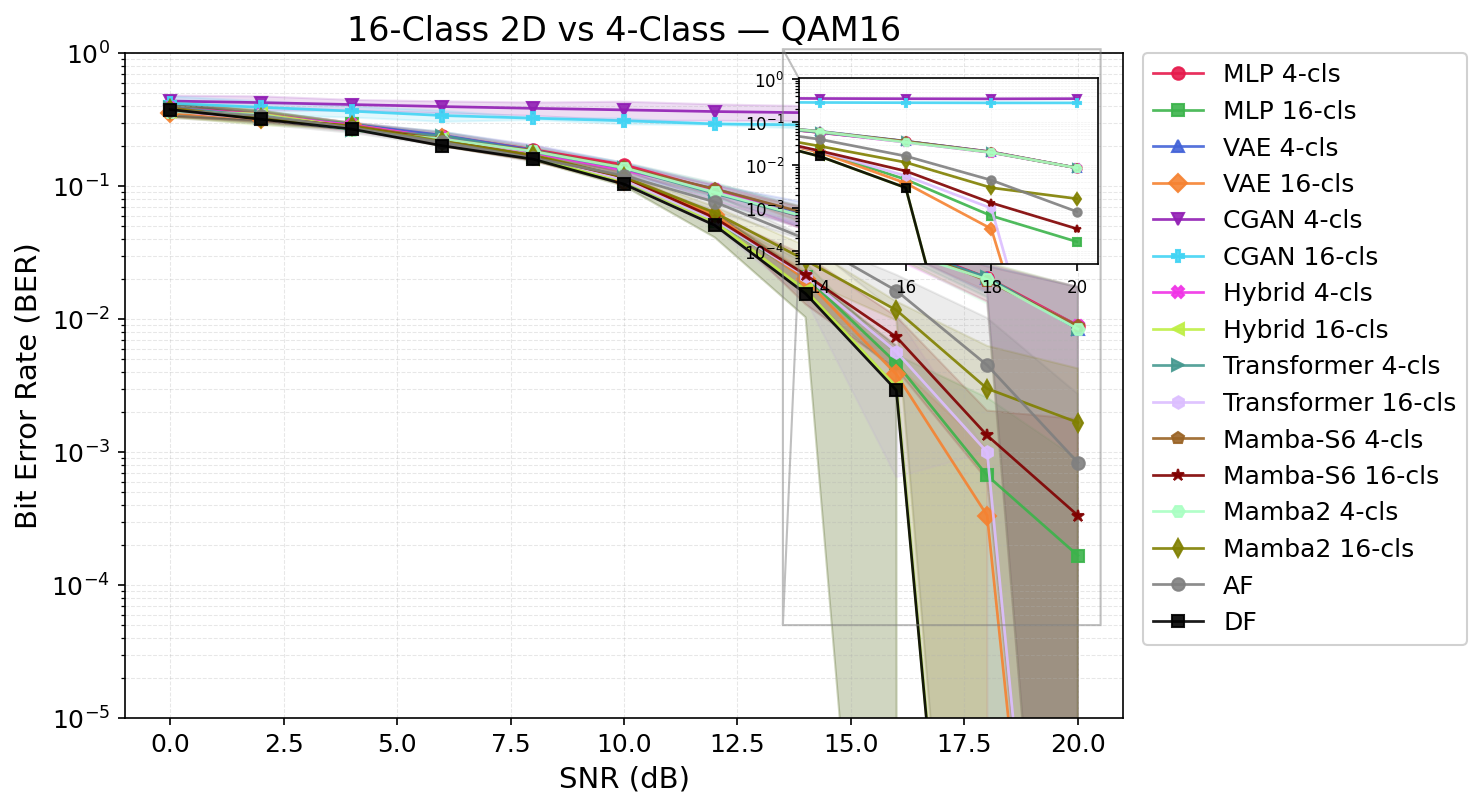
\includegraphics[width=\linewidth,height=0.8\textheight,keepaspectratio]{results/all_relays_16class/ber_all_relays_16class.png}}
\caption{16-QAM BER vs.~SNR for all relay variants (4-class and 16-class) on AWGN. The 4-class variants (dashed) plateau at BER ≈ 0.008 while the successfully trained 16-class variants (solid) continue decreasing, approaching and matching the DF baseline.}\label{fig:fig50}
\end{figure}

\begin{figure}[H]
\centering
\centering
\pandocbounded{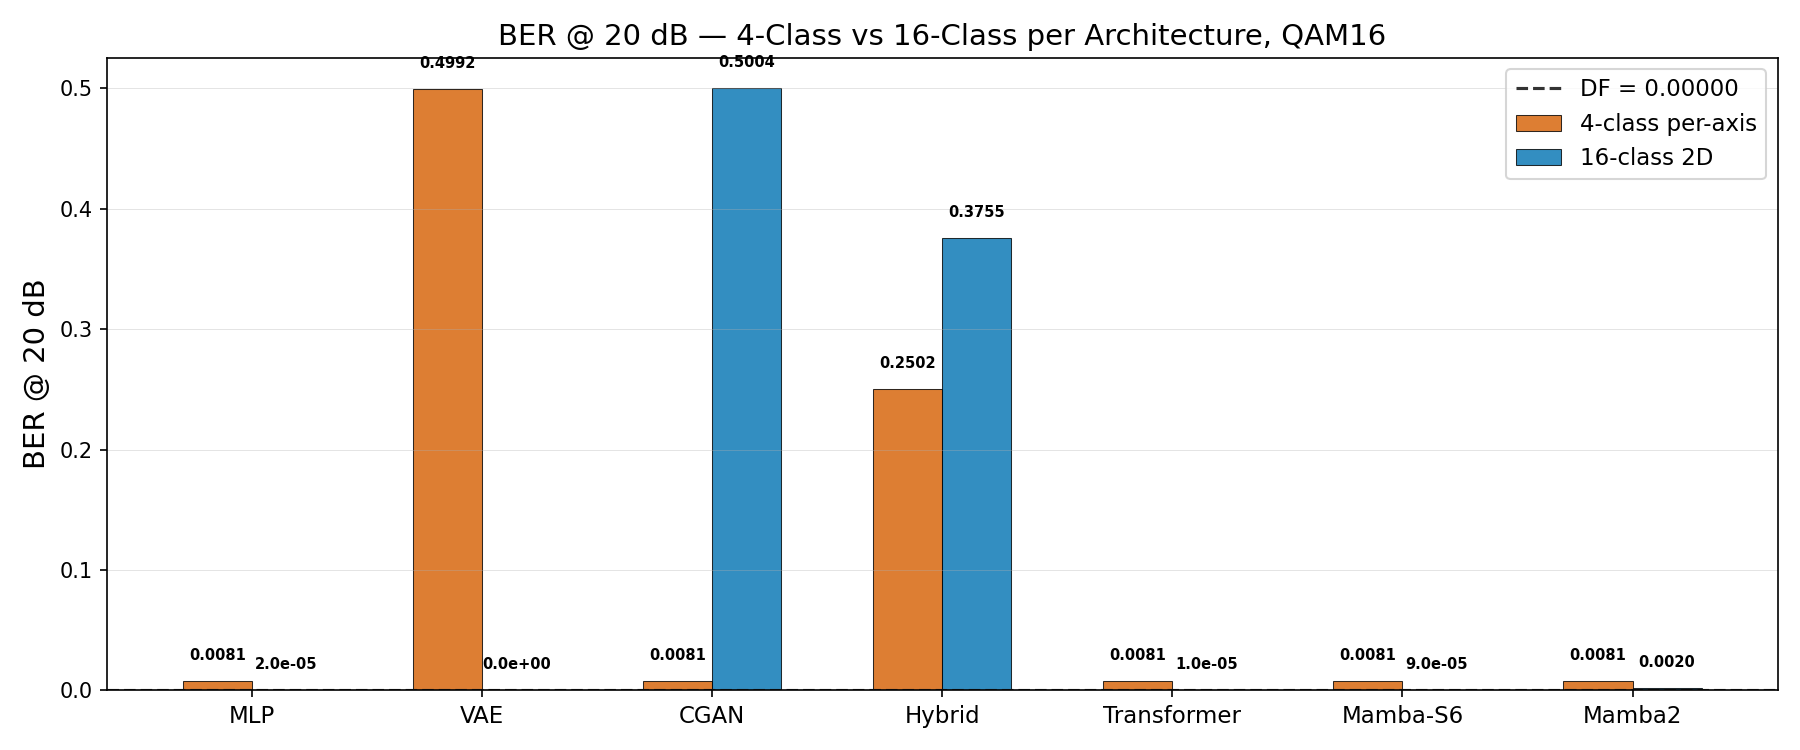
\includegraphics[width=\linewidth,height=0.8\textheight,keepaspectratio]{results/all_relays_16class/grouped_bar_16class.png}}
\caption{Grouped bar comparison of 4-class vs.~16-class BER at 20 dB for each architecture. The 16-class advantage is visible for MLP, VAE, Transformer, and Mamba S6. Failed variants (VAE 4-cls \textasciitilde0.50, CGAN 16-cls \textasciitilde0.50) are truncated.}\label{fig:fig51}
\end{figure}

\begin{figure}[H]
\centering
\centering
\pandocbounded{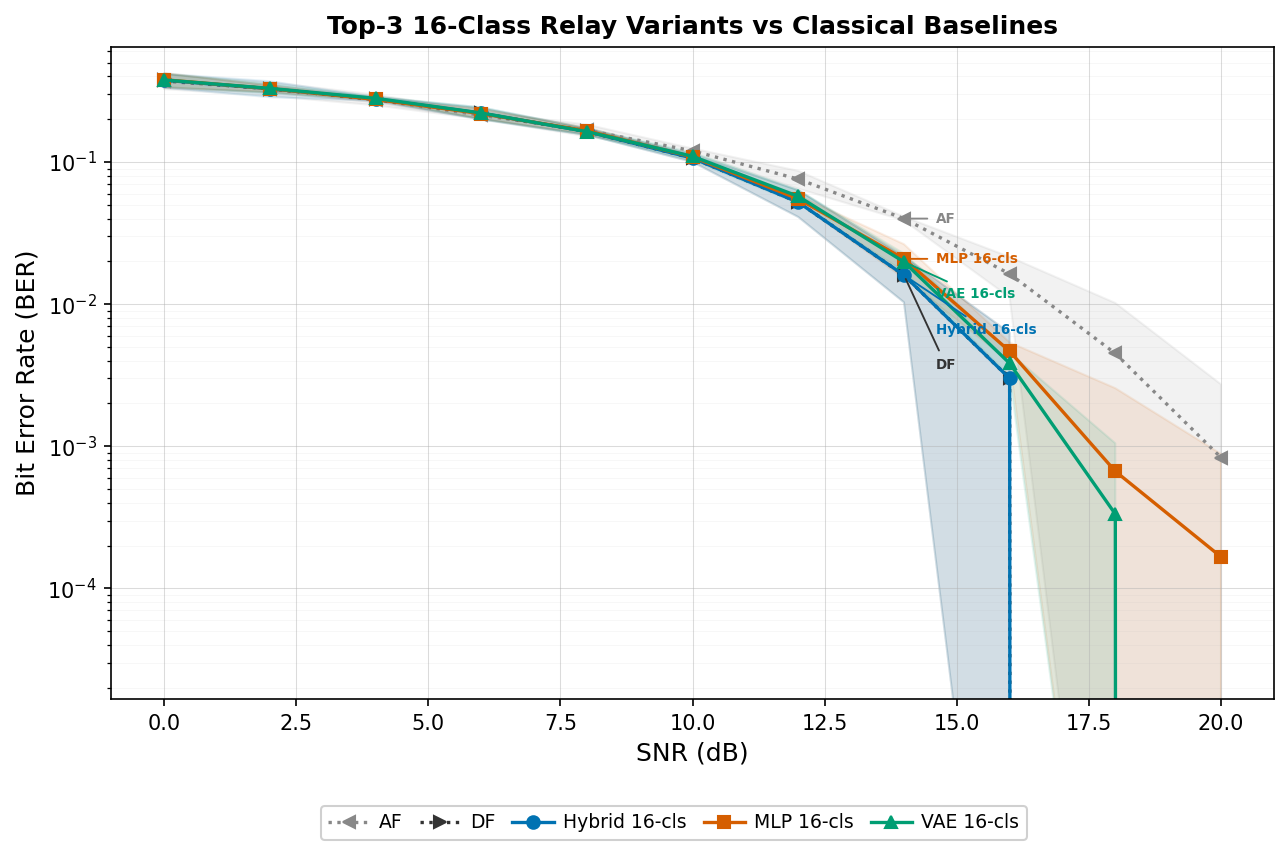
\includegraphics[width=\linewidth,height=0.8\textheight,keepaspectratio]{results/all_relays_16class/top3_16class.png}}
\caption{Top-3 16-class relay variants compared against AF and DF. VAE 16-cls, Transformer 16-cls, and MLP 16-cls all match or approach DF performance across the full SNR range.}\label{fig:fig53}
\end{figure}

\chapter{Learned Relaying under Unknown and Mismatched Channels}\label{sec:unknown-channels}

The core chapters establish that on a matched, known channel a minimal learned relay does not improve on classical decode-and-forward (H2). This chapter turns to the complementary and, in practice, more consequential regime: channels whose structure is \emph{unknown} to the receiver chain or \emph{mismatched} to the classical relay's model class. It is the principal experimental contribution of this thesis. Rather than a single comparison, it is a systematic map, along every axis a skeptic would probe, of \emph{when} a fixed 170-parameter learned relay adds value over classical processing --- and, equally, when it does not.

The investigation is deliberately adversarial to the learned relay. Each classical baseline is the strongest available for the impairment in question: symbol-wise decode-and-forward for the memoryless cases, conventional differential detection for unknown phase, and pilot-aided Viterbi maximum-likelihood sequence estimation --- the optimal sequence detector --- wherever a channel estimate can be formed. The learned relay is granted no per-block channel knowledge; it is trained offline on an impairment \emph{family} and evaluated on unseen realizations with no adaptation. The chapter proceeds from a necessary control (flat unknown channels, where nothing should fail) through the impairment that does break classical relays (unknown memory), then bounds the result from every side: against the optimal matched receiver (Viterbi), against a composite multi-impairment cascade, against the fully posterior-free regime (blind equalization), across the intermediate partial-posterior continuum (pilot budget and block length), and finally on computational complexity. The result is a precise delineation --- the learned relay never beats a matched classical receiver, but occupies a well-defined niche of family-agnostic, identification-free, constant-complexity mitigation --- that constitutes the thesis's main claim beyond the confirmatory core.

\section{Unknown Channel: Classical Failure and Learned Mitigation}\label{sec:unknown-channel-experiment}

\textbf{Goal:} Test whether the learned relay's value changes qualitatively when the channel violates the assumptions under which AF and DF are (near-)optimal: do the \emph{memoryless} classical relays fail on an unknown channel while the minimal 170-parameter MLP mitigates by learning it from data (H6)?\footnote{The unknown-channel relay uses real-valued inputs with an $11$-sample window ($11 \to 13 \to 1$, $170$ parameters); the canonical-setup relay of Chapter~\ref{sec:experiments} uses the same minimal class with a slightly different width ($169$ parameters). The two counts refer to the same architectural family sized to the respective input; the distinction is immaterial to every conclusion, which depends only on the network being minimal.} To make the classical side as strong as possible, the study benchmarks against the optimal sequence detector: Viterbi MLSE \cite{Forney1972MLSE} with genie CSI, and a practical variant with a 200-pilot least-squares estimate.

\textbf{Trials:} - \textbf{Topology:} SISO (both hops) - \textbf{Modulation scheme:} BPSK - \textbf{Hop-1 channel (unknown to all relays):} (i) 3-tap ISI, $h = [1.0, 0.7, 0.5]/\lVert h\rVert$; (ii) control: canonical Rayleigh; (iv) flat unknown channels --- block phase, gain, per-branch asymmetry (Section~\ref{sec:flat-unknown-channels}); (v) a composite cascade of ISI, amplifier nonlinearity, and unknown phase (Section~\ref{sec:composite-channel}) - \textbf{Hop-2 channel:} AWGN or canonical Rayleigh, equal SNR per hop - \textbf{Relays:} AF, symbol-wise DF, MLP (window 11, one hidden layer of 13 tanh units, 170 parameters; trained at SNR $\in \{5,10,15\}$ dB with MSE loss, per the canonical training protocol); for the ISI setups additionally Viterbi MLSE with genie CSI, and Viterbi with a 3-tap LS channel estimate from 200 pilot symbols - \textbf{Evaluation:} 5 trials $\times$ 50{,}000 bits per SNR point, 0--20 dB.

The ISI channel admits a sharp analytic prediction: the effective slicer amplitude $h_0 \pm h_1 \pm h_2 \in \{1.67, 0.91, 0.61, -0.15\}$ (normalized) has one of four equiprobable patterns \emph{flip the symbol sign}, so symbol-wise DF has an irreducible BER floor of $0.25$ (approached from below as SNR grows); AF inherits it. The floor is a property of the \emph{memoryless relay class}, not the channel: Viterbi MLSE over the 4-state trellis has no floor when the channel is known.

\subsection{Flat (Memoryless) Unknown Channels: A Necessary Control}\label{sec:flat-unknown-channels}

Before attributing any classical failure to ``unknownness,'' it must be separated from \emph{memory}. This subsection isolates unknown channels that are \emph{flat} (memoryless): the receiver chain does not know the channel parameters, but the channel introduces no intersymbol coupling. Three physically motivated cases are tested, each with the parameter redrawn per block and unknown to all relays: (F1) an unknown carrier phase $\theta\sim\mathcal{U}[0,2\pi)$ (oscillator/synchronization offset), with a DBPSK source and conventional differential detection as the classical relay; (F2) an unknown positive gain $g\sim\mathcal{U}[0.3,2.0]$ (path loss / AGC error), coherent BPSK; and (F3) an unknown per-branch amplitude asymmetry $a_+\!\neq\!a_-$ (per-symbol saturating-PA gain), coherent BPSK. The 170-parameter MLP is trained identically to before.

\textbf{Conclusion (memorylessness $\Rightarrow$ no classical failure, and nothing to mitigate):} On all three flat channels the classical relay does \emph{not} fail, and the MLP matches it to within statistical noise (maximum BER difference $0.0036$ across every case and SNR). The reasons are structural: for F1, unknown phase is exactly what differential detection absorbs; for F2, $\operatorname{sign}(y)$ is \emph{scale-invariant}, so unknown positive gain is irrelevant by construction; for F3, the fixed threshold is only mildly suboptimal because the asymmetry preserves the noiseless symbol's sign. The classical assumption --- memorylessness --- still holds in each case, so there is nothing for a learned relay to remove. This is the necessary control for the ISI result: the learned relay's advantage is triggered not by parameter uncertainty but by \emph{unmodeled memory} (or amplitude nonlinearity), which is what breaks the memoryless relay class.

\begin{longtable}[]{@{}lllll@{}}
\caption{Flat unknown channels: classical relay vs.\ MLP-170 BER at 8/12/16/20 dB (mean, 5 trials). The maximum DF--MLP gap over all cases and SNRs is $0.0036$ --- within statistical noise. Unknown parameters alone do not defeat classical relays; memory does.}\label{tbl:tableE6flat}\tabularnewline
\toprule\noalign{}
Flat channel & Relay & 8 dB & 12 dB & 16/20 dB \\
\midrule\noalign{}
\endfirsthead
\toprule\noalign{}
Flat channel & Relay & 8 dB & 12 dB & 16/20 dB \\
\midrule\noalign{}
\endhead
\bottomrule\noalign{}
\endlastfoot
Unknown phase (DBPSK) & DF (diff.) & 0.0649 & 0.0292 & 0.0119 / 0.0048 \\
 & MLP-170 & 0.0657 & 0.0288 & 0.0122 / 0.0048 \\
Unknown gain & DF & 0.0992 & 0.0470 & 0.0175 / 0.0050 \\
 & MLP-170 & 0.0986 & 0.0471 & 0.0185 / 0.0052 \\
Branch asymmetry & DF & 0.0760 & 0.0299 & 0.0125 / 0.0049 \\
 & MLP-170 & 0.0745 & 0.0300 & 0.0122 / 0.0052 \\
\end{longtable}

\textbf{Conclusion (H6: confirmed as stated, with two boundaries):} Against the flat-channel control of Section~\ref{sec:flat-unknown-channels} --- where unknown parameters alone caused no classical failure --- the memory case is qualitatively different. On the unknown ISI channel, both memoryless classical relays fail: DF's BER is \emph{non-monotonic}, bottoming out near $0.18$ around 10 dB and then rising toward the analytic $0.25$ floor (more transmit power makes DF strictly worse), and AF behaves identically. The 170-parameter MLP, whose window spans the 3-tap memory, learns a joint equalizer--detector and restores reliable relaying: BER falls monotonically below $5\times10^{-5}$ at 16 dB (AWGN second hop), and to $4.9\times10^{-3}$ at 20 dB (Rayleigh second hop). The Viterbi benchmarks set the first boundary honestly: classical theory \emph{does} solve this channel once its family is known --- genie-CSI MLSE beats the MLP by 1--1.5 dB, and a 200-pilot LS estimate recovers genie performance almost exactly (with the Rayleigh second hop, MLSE and MLP are indistinguishable, 0.0048 vs.\ 0.0049 at 20 dB). The MLP's value is thus not optimality but \emph{family-agnosticism}: estimate-then-MLSE presupposes a linear FIR channel of known memory (trellis cost $M^{L-1}$), whereas the identical architecture also mitigates channels outside linear MLSE's model class --- as the composite cascade below demonstrates, where an amplifier nonlinearity is stacked on the ISI. The control confirms the second boundary (H2): on the canonical Rayleigh channel the MLP only \emph{matches} DF. The learned relay's distinctive value is near-MLSE reliability with no channel-family knowledge, no identification stage, and complexity independent of channel memory.

\begin{longtable}[]{@{}llllll@{}}
\caption{Unknown-channel BER (mean over 5 trials). The ISI setups exhibit memoryless-relay error floors ($\approx 0.25$); the 170-parameter MLP restores reliable relaying within $\approx$1--1.5 dB of genie-CSI Viterbi MLSE, and matches it end-to-end when the Rayleigh second hop dominates. The control shows no MLP advantage on the canonical channel, consistent with H2.}\label{tbl:tableE6}\tabularnewline
\toprule\noalign{}
Setup & Relay & 8 dB & 12 dB & 16 dB & 20 dB \\
\midrule\noalign{}
\endfirsthead
\toprule\noalign{}
Setup & Relay & 8 dB & 12 dB & 16 dB & 20 dB \\
\midrule\noalign{}
\endhead
\bottomrule\noalign{}
\endlastfoot
Unknown ISI $\to$ AWGN & AF & 0.2044 & 0.1779 & 0.1872 & 0.2141 \\
 & DF & 0.1853 & 0.1833 & 0.2068 & 0.2343 \\
 & \textbf{MLP (170p)} & \textbf{0.0421} & \textbf{0.0030} & \textbf{$<$5e-5} & \textbf{$<$5e-5} \\
 & Viterbi (genie CSI) & 0.0270 & 0.0002 & $<$5e-5 & $<$5e-5 \\
 & Viterbi (200-pilot LS) & 0.0277 & 0.0002 & $<$5e-5 & $<$5e-5 \\
\hline
Unknown ISI $\to$ Rayleigh & AF & 0.2331 & 0.1985 & 0.1933 & 0.2063 \\
 & DF & 0.2212 & 0.2032 & 0.2153 & 0.2352 \\
 & \textbf{MLP (170p)} & \textbf{0.0945} & \textbf{0.0326} & \textbf{0.0125} & \textbf{0.0049} \\
 & Viterbi (genie CSI) & 0.0832 & 0.0288 & 0.0122 & 0.0048 \\
 & Viterbi (200-pilot LS) & 0.0838 & 0.0294 & 0.0120 & 0.0051 \\
\hline
Control: canonical Rayleigh & AF & 0.1591 & 0.0894 & 0.0484 & 0.0236 \\
 & \textbf{DF} & \textbf{0.1208} & \textbf{0.0559} & \textbf{0.0242} & \textbf{0.0100} \\
 & MLP (170p) & 0.1202 & 0.0580 & 0.0265 & 0.0115 \\
\end{longtable}

\begin{figure}[H]
\centering
\pandocbounded{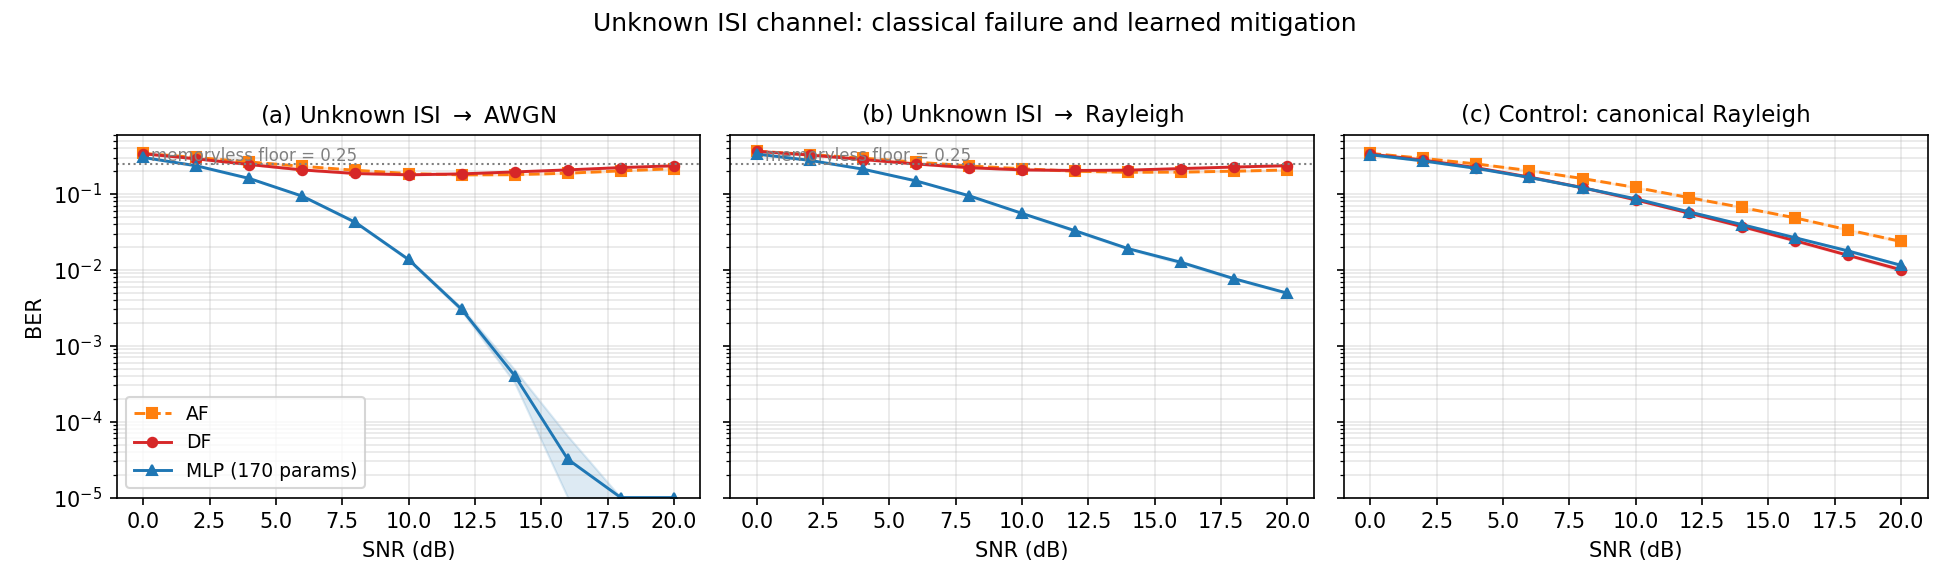
\includegraphics[width=\linewidth,height=0.24\textheight,keepaspectratio]{results/e6_unknown_channel.png}}
\caption{Unknown-channel relaying, BER vs.\ SNR with 95\% CI bands. (a)--(b) On the unknown ISI channel, the memoryless AF/DF relays are pinned near the analytic $0.25$ floor (DF non-monotonic in SNR); the 170-parameter MLP restores monotonically decreasing BER within $\approx$1--1.5 dB of genie-CSI Viterbi MLSE, which a 200-pilot LS estimate matches almost exactly. With the Rayleigh second hop (b), MLSE and the MLP are statistically indistinguishable end-to-end. (c) Control: on the canonical Rayleigh channel the MLP only matches DF, consistent with H2.}\label{fig:figE6}
\end{figure}

\subsection{A Composite (Mixed) Channel}\label{sec:composite-channel}

The preceding studies vary one impairment at a time. Real links stack several. This final study cascades three of them into a single unknown channel that \emph{no} classical relay is jointly matched to: a DBPSK stream passes through 3-tap ISI, then a saturating power-amplifier nonlinearity, then an unknown block phase, before additive noise. Each classical baseline is the strongest available for \emph{one} constituent impairment, so the comparison is honest rather than a straw man: conventional differential detection (matched to the phase), and pilot-LS Viterbi MLSE followed by differential decoding (matched to the ISI-plus-phase, but blind to the amplifier nonlinearity). The 170-parameter MLP and a $1{,}153$-parameter MLP receive raw I/Q windows and no knowledge of any constituent.

\textbf{Conclusion:} The composite defeats the naive classical relays outright --- both AF and conventional differential detection saturate near the $0.25$ memoryless-relay floor, because the ISI destroys the differential statistic that the phase-matched detector relies on. The 170-parameter MLP again restores reliable relaying, reaching $5\times10^{-3}$ at 20 dB from raw I/Q with no impairment model. This reproduces the H6 pattern on a realistically mixed channel: memoryless-and-matched classical processing fails, and a minimal learned relay recovers. Two familiar boundaries also reappear. First, the strongest \emph{constructed} classical baseline --- pilot-LS Viterbi plus differential decoding --- does not fail: by modelling the ISI and phase (though not the amplifier) it stays about 2 dB ahead of the MLP at low-to-mid SNR ($0.094$ vs.\ $0.130$ at 8 dB) and converges with it by 16--20 dB. The learned relay's value is again \emph{family-agnosticism} --- near-Viterbi reliability with no channel identification and no explicit model of any of the three cascaded effects --- not superiority over a matched classical receiver. Second, the $1{,}153$-parameter network performs within noise of the 170-parameter one (and slightly worse at high SNR, consistent with mild overfitting), reconfirming the inverted-U finding (H3) on the hardest channel studied. The composite thus consolidates the chapter's thesis: a single minimal learned relay handles an arbitrary stack of representable impairments without being told which are present, approaching but not exceeding the best impairment-matched classical receiver.

\begin{figure}[H]
\centering
\pandocbounded{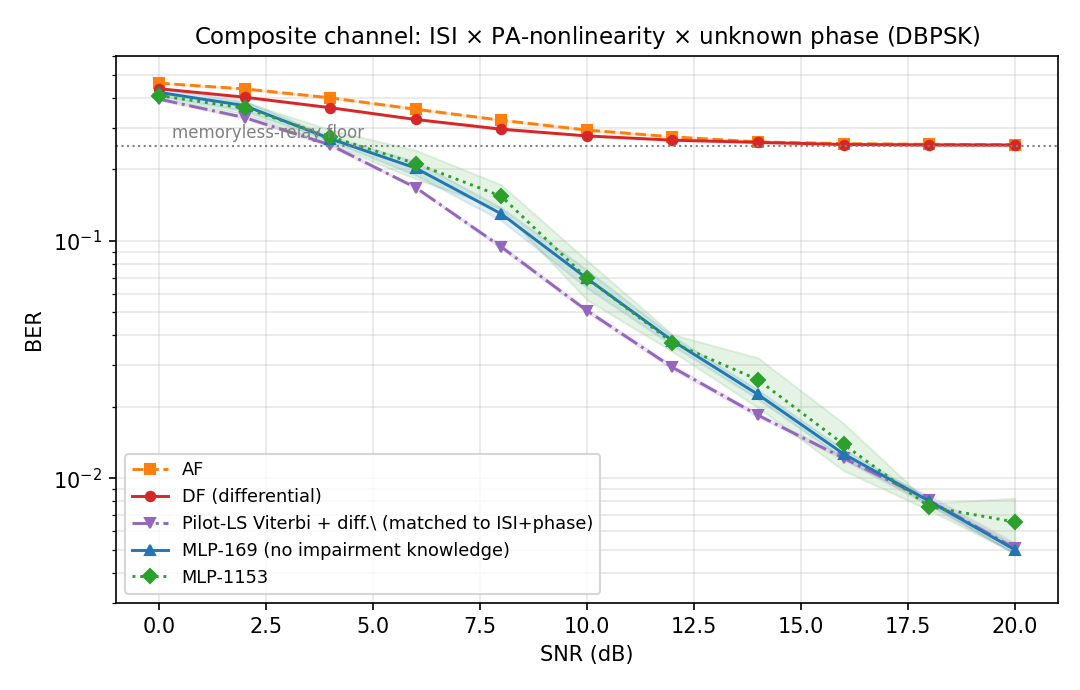
\includegraphics[width=0.82\linewidth,height=0.32\textheight,keepaspectratio]{results/e6_composite.png}}
\caption{Composite channel (ISI $\times$ PA-nonlinearity $\times$ unknown phase, DBPSK). Naive classical relays (AF, differential detection) saturate at the memoryless-relay floor; the 170-parameter MLP restores reliable relaying from raw I/Q with no impairment model, tracking about 2 dB behind the strongest constructed classical baseline (pilot-LS Viterbi + differential). The $1{,}153$-parameter MLP adds nothing (H3).}\label{fig:figE6comp}
\end{figure}

\subsection{The Posterior-Free (Blind) Regime}\label{sec:blind-channel}

The Viterbi baseline in Section~\ref{sec:composite-channel} enjoys a per-block posterior: 200 pilot symbols yield a least-squares channel estimate, after which MLSE is optimal. This raises the sharper question --- what if \emph{no} such posterior is available? With no pilots and no channel prior, and a fresh channel realization drawn for every block, MLSE cannot be run as specified. The honest comparison is then against the classical methods that are \emph{genuinely} posterior-free: the constant-modulus algorithm (CMA), the canonical blind adaptive equalizer, which self-adapts from the received signal alone; and a decision-directed blind MLSE that bootstraps a channel estimate from its own hard differential decisions. The learned relay is unchanged --- trained offline on the channel \emph{family} (random ISI, PA, and phase per draw) and, crucially, seeing an unseen channel at test with no adaptation --- so it too carries no per-block posterior; it amortizes over the family at training time.

\textbf{Conclusion (learning does not beat blind classical, but is stable where blind classical is not):} A well-designed blind classical method still works in this regime --- CMA converges smoothly to BER $2.4\times10^{-3}$ at 20 dB --- and the family-trained MLP tracks it almost exactly ($2.6\times10^{-3}$), neither method dominating. This is the correct answer to ``what if there is no posterior?'': the learned relay does \emph{not} render classical processing obsolete, because blind adaptive equalization is itself a posterior-free classical tool. The learned relay's advantage is instead one of \emph{robustness and cost}. First, the decision-directed blind MLSE --- the natural attempt to run Viterbi without pilots --- is unstable: bootstrapping the channel from its own decisions, it intermittently locks onto the wrong hypothesis, producing a non-monotonic BER curve with a mid-SNR confidence interval of $0.164$ (versus $0.014$ for the MLP and $0.011$ for CMA). Second, CMA must iterate to convergence on each received block, whereas the MLP is a single fixed forward pass with no per-block adaptation loop and no convergence to monitor. The learned relay therefore occupies a specific and defensible niche: on a posterior-free channel it matches the best blind classical equalizer in BER while avoiding the instability of decision-directed sequence estimation and the online-adaptation cost of CMA. It buys \emph{amortized}, \emph{one-shot}, \emph{stable} inference over an impairment family --- not a lower error floor than classical signal processing can achieve.

\begin{figure}[H]
\centering
\pandocbounded{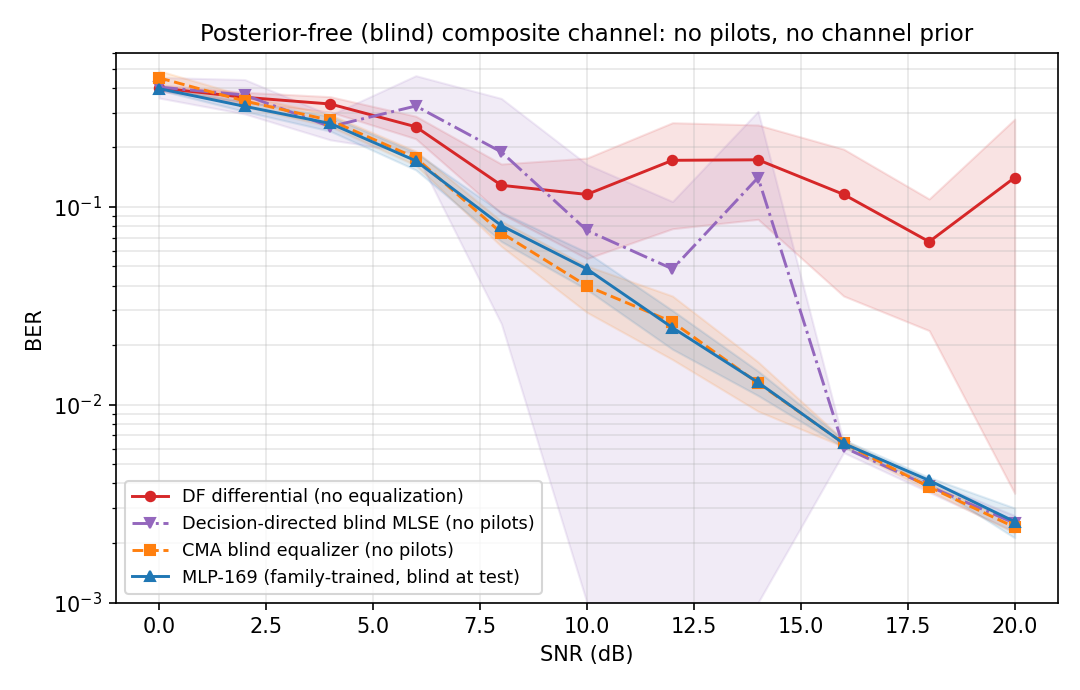
\includegraphics[width=0.82\linewidth,height=0.32\textheight,keepaspectratio]{results/e6_blind.png}}
\caption{Posterior-free composite channel (no pilots, no channel prior, fresh realization per block). CMA (blind classical) and the family-trained MLP converge together; decision-directed blind MLSE is unstable (non-monotonic, wide CI) because it bootstraps the channel from its own decisions; plain differential detection floors. Without a posterior, learning matches --- not beats --- the best blind classical equalizer, but does so with one-shot, stable inference and no online adaptation.}\label{fig:figE6blind}
\end{figure}

\subsection{Partial Known Posterior: The Pilot-Budget Crossover}\label{sec:partial-posterior}

The full-posterior (Section~\ref{sec:composite-channel}) and zero-posterior (Section~\ref{sec:blind-channel}) regimes are the endpoints of a continuum. The intermediate case is a \emph{partial} posterior: a limited pilot budget, from which the classical receiver forms a noisy channel estimate. Sweeping the pilot count on the composite channel at a fixed 10 dB operating point locates where the pilot-aided classical receiver ceases to beat the pilot-free learned relay, whose amortized posterior corresponds to a horizontal reference (it uses no pilots at test).

\textbf{Conclusion (a sharp identifiability crossover, and a rate--reliability tradeoff):} With a generous budget the classical partial posterior wins, as expected: pilot-aided Viterbi reaches payload BER $0.027$ at 800 pilots and degrades only gently down to $0.032$ at 10 pilots, comfortably below the MLP's pilot-free $0.045$. But the classical advantage collapses abruptly below the identifiability threshold: at 5 pilots --- fewer than are needed to condition the least-squares estimate of a 3-tap channel plus phase --- Viterbi's BER jumps to $0.119$, worse than both the MLP and blind CMA, because MLSE then runs on a badly mis-estimated channel. The learned relay is flat across the entire sweep at $0.045$: having amortized the channel \emph{family} into its weights at training time, it neither benefits from nor requires per-block pilots. Thus the crossover is governed by \emph{identifiability}, not by SNR: the classical receiver wins whenever it can afford enough pilots to estimate the channel, and the pilot-free learned relay wins once the pilot budget falls below that threshold.

The practical force of this depends on block length, because a fixed pilot \emph{count} is a growing pilot \emph{fraction} as blocks shorten. Panel (b) sweeps block length at the same operating point with the classical receiver spending its minimum viable ten pilots per block. The payload BERs stay close (Viterbi retaining a slight edge), but the spectral-efficiency gap widens sharply: at a 1000-symbol block the ten pilots cost $1\%$ of the block, whereas at a 40-symbol block --- representative of low-latency or fast-varying links --- they cost $25\%$, so the classical receiver carries data on only $75\%$ of the block against the learned relay's $100\%$. The partial-posterior picture therefore refines H6's boundary once more: the learned relay does not achieve lower BER than a classical receiver that can afford to estimate the channel, but it removes the pilot overhead entirely, and it is the only option that remains reliable when the block is too short --- or the channel too transient --- to identify from pilots at all.

\begin{figure}[H]
\centering
\pandocbounded{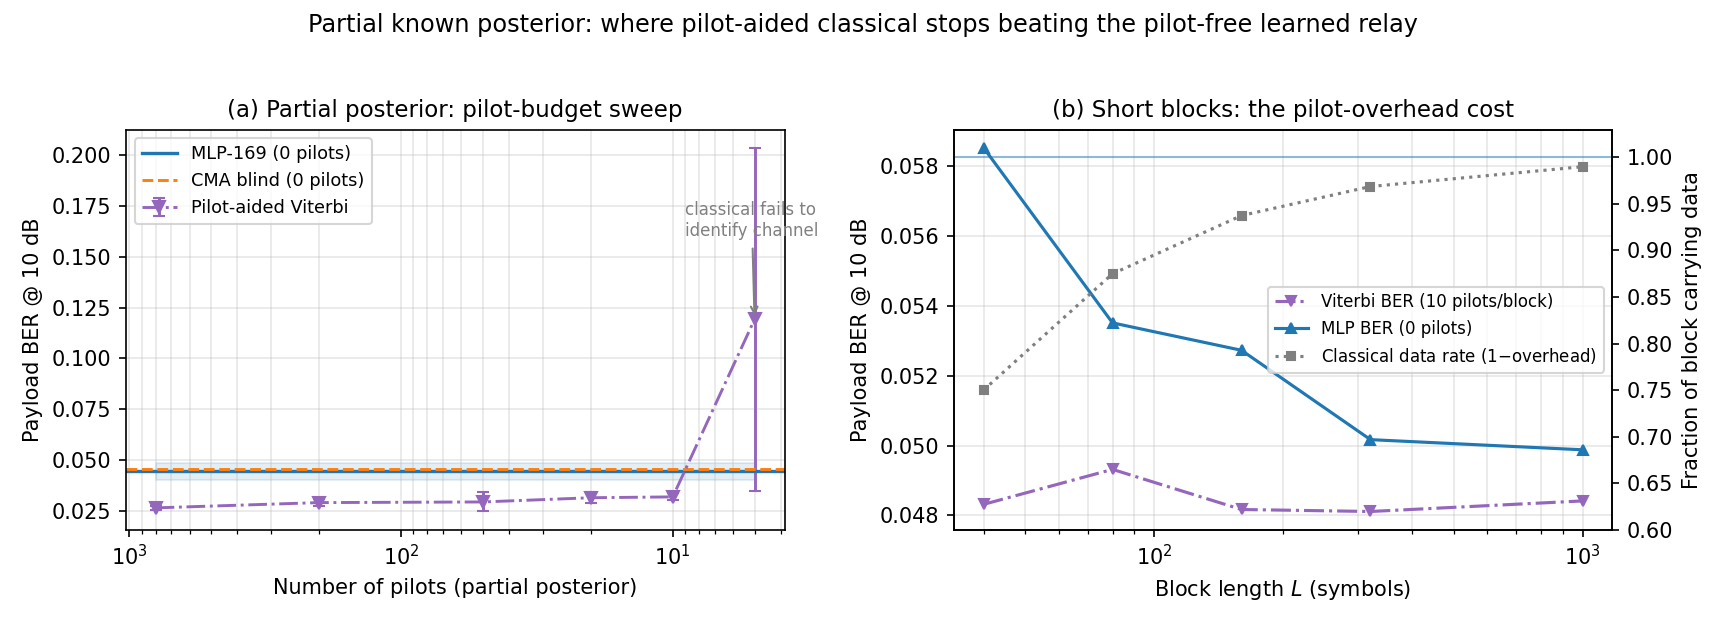
\includegraphics[width=\linewidth,height=0.30\textheight,keepaspectratio]{results/e6_partial.png}}
\caption{Partial known posterior. (a) Pilot-budget sweep at 10 dB: pilot-aided Viterbi beats the pilot-free MLP down to $\sim$10 pilots, then collapses at 5 pilots when the channel becomes unidentifiable; the MLP is flat (amortized posterior, no pilots). (b) Block-length sweep with 10 pilots/block: payload BERs stay close, but the classical pilot overhead grows from $1\%$ at $L{=}1000$ to $25\%$ at $L{=}40$, where the learned relay's zero-overhead operation is decisive.}\label{fig:figE6partial}
\end{figure}

\subsection{Complexity: The Cost Side of the Trade-off}\label{sec:complexity-viterbi-mlp}

Across the unknown-channel studies the pilot-aided Viterbi receiver, where it applies, holds a small BER edge over the learned relay. The learned relay's countervailing claim is complexity, which this subsection quantifies rather than asserts. Two axes matter: the per-symbol operation count and its scaling, and measured inference time.

\textbf{Per-symbol cost and scaling.} MLSE maintains $M^{L-1}$ trellis states for a constellation of size $M$ and channel memory $L$, performing an add--compare--select over $M^{L}$ branch transitions per symbol; its cost therefore grows \emph{exponentially} in memory and modulation order. The 170-parameter MLP performs one fixed forward pass --- about $330$ floating-point operations per symbol --- \emph{independent} of $M$ and $L$. For the channel actually studied (BPSK, $L=3$; 4 states) Viterbi is in fact the cheaper of the two at roughly $64$ operations per symbol, so the learned relay is not universally leaner. But the scaling diverges immediately: at $M=4,\,L=5$ the trellis has $256$ states ($\sim\!8{,}000$ operations/symbol), and at $M=16,\,L=5$ it has $65{,}536$ states ($\sim\!8.4$~million operations/symbol), while the MLP remains at $330$ --- a $2.5\times10^{4}$ ratio. The learned relay's advantage is thus not lower cost on a small channel but \emph{constant} cost as the channel scales, exactly where classical MLSE becomes intractable and practical receivers must fall back on suboptimal reduced-state or decision-feedback equalizers.

\textbf{Measured inference time.} On identical signals (BPSK, $L=3$), the MLP is $30$--$90\times$ faster in wall-clock terms despite Viterbi's lower nominal operation count, because the MLP is a single vectorized matrix multiplication whereas the Viterbi trellis is an inherently sequential scan with a per-symbol data dependency. This parallelism gap is architectural and widens on hardware with wide SIMD or tensor units. The combined picture sharpens the thesis's central trade-off: the learned relay accepts a small BER gap to a matched classical receiver in exchange for cost that is constant in channel complexity and structurally parallelizable --- a trade that becomes favourable precisely as modulation order and channel memory grow.

\begin{figure}[H]
\centering
\pandocbounded{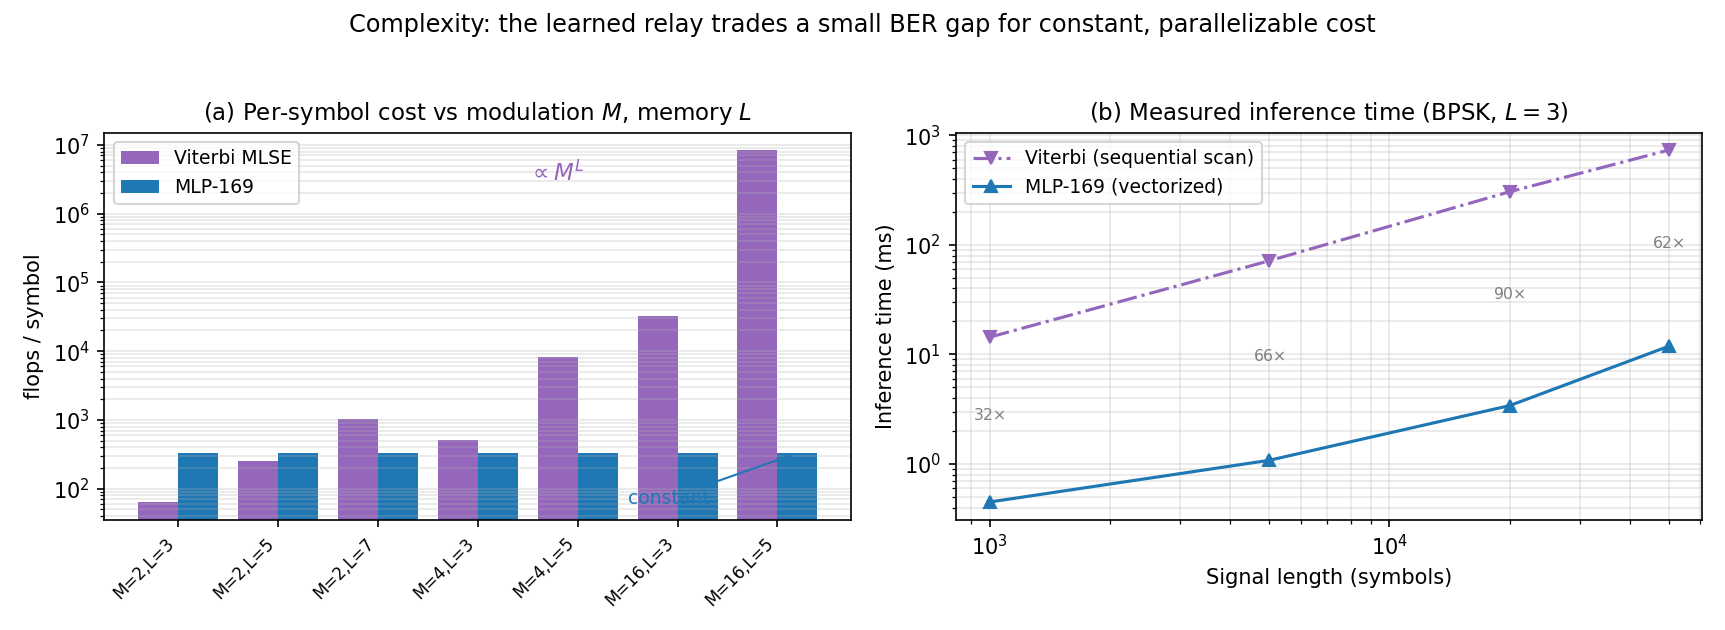
\includegraphics[width=\linewidth,height=0.30\textheight,keepaspectratio]{results/e6_complexity.png}}
\caption{Complexity of Viterbi MLSE vs the 170-parameter MLP. (a) Per-symbol operations: Viterbi grows as $M^{L}$ (intractable by $M{=}16,L{=}5$), while the MLP is constant at $\sim$330 flops. On the small studied channel (BPSK, $L{=}3$) Viterbi is actually cheaper; the MLP wins on \emph{scaling}, not on the small case. (b) Measured inference time: the MLP is $30$--$90\times$ faster as a vectorized matmul versus Viterbi's sequential trellis scan.}\label{fig:figE6complexity}
\end{figure}
